\chapter{Finite Markov Chains}

When a stochastic process $\left(X_{\alpha} \right)_{\alpha \in \Az}$ is not independent it is said to be dependent.  
So far we have mostly concerned ourselves with independent processes.  
In this chapter we introduce finite Markov chains and their  simulation methods.
Finit Markov chains are among the simplest stochastic processes with a `first-order' dependence called Markov dependence.

\section{Introduction}\label{S:FiniteMCIntro}
A finite Markov chain is a stochastic process that moves among elements in a finite set $\Xz$ as follows: when at $x \in \Xz$ the next position is chosen at random according to a fixed probability distribution $P(\cdot | x)$.  We define such a process more formally below.

\begin{definition}[Finite Markov Chain]\label{D:TimeHomFiniteMC}
A stochastic sequence, $$\left(X_n\right)_{n \in \Zz_+} := (X_0,X_1,\ldots),$$ is a homogeneous {\bf Markov chain} with {\bf state space} $\Xz$ and {\bf transition matrix} $P:=\left(P(x,y)\right)_{(x,y)\in \Xz^2}$ if for all pair of {\bf states} ${(x,y)\in \Xz^2 := \Xz \times \Xz}$, all integers $t \geq 1$, and all probable historical events $H_{t-1} := \bigcap_{n=0}^{t-1} \{ X_n = x_n \}$ with $\p \left(H_{t-1} \cap \{X_t = x\} \right) > 0$, the following {\bf Markov property} is satisfied: 
\begin{equation}\label{E:FiniteMarkovProperty}
\p\left(X_{t+1} = y | H_{t-1} \cap \{X_t = x\} \right)=\p\left(X_{t+1} = y | X_t = x \right) =: P(x,y) \enspace .
\end{equation}
\end{definition}
The Markov property means that the conditional probability of going to state $y$ at time $t+1$ from state $x$ at current time $t$ is always given by the $(x,y)$-th entry $P(x,y)$ of the transition matrix $P$, no matter what sequence of states $(x_0,x_1,\ldots,x_{t-1})$ preceded the current state $x$.  Thus, the $|\Xz| \times |\Xz|$ matrix $P$ is enough to obtain the state transitions since the $x$-th row of $P$ is the probability distribution $P(x,\cdot) := \left( P(x,y) \right)_{y \in \Xz}$.  For this reason $P$ is called a {\bf stochastic matrix}, i.e.,
\begin{equation}\label{E:StochasticMatrixConds}
P(x,y) \geq 0 \quad \text{for all } (x,y) \in \Xz^2 \qquad \text{and} \quad \sum_{y \in \Xz} P(x,y) = 1 \quad \text{for all } x \in \Xz \enspace .
\end{equation}
Thus, for a Markov chain $\left(X_n\right)_{n \in \Zz_+}$, the distribution of $X_{t+1}$ given $X_0,\ldots,X_t$  depends on $X_t$ alone. Because of this dependence on the previous state, the stochastic sequence, $(X_0,X_1,\ldots)$, are {\it not} independent.  We introduce the most important concepts using a simple example.

\begin{example}[Flippant Freddy]\label{EX:FlippantFreddy}
Freddy the flippant frog lives in an enchanted pond with only two lily pads, {\em rollopia} and {\em flipopia}.  A wizard gave a  die and a silver coin to help flippant Freddy decide where to jump next.  Freddy left the die on rollopia and the coin on flipopia.  When Freddy got restless in rollopia he would roll the die and if the die landed odd he would leave the die behind and jump to flipopia, otherwise he would stay put.  When Freddy got restless in flipopia he would flip the coin and if it landed Heads he would leave the coin behind and jump to rollopia, otherwise he would stay put.

Let the state space $\Xz=\{r,f\}$, and let $(X_0, X_1,\ldots)$ be the sequence of lily pads occupied by Freddy after his restless moments.  Say the die on rollopia $r$ has probability $p$ of turning up odd and the coin on flipopia $f$ has probability $q$ of turning up heads.  We can visualise the rules of Freddy's jumps by the following {\bf transition diagram}:
\begin{figure}[htpb]
\caption{Transition Diagram of Flippant Freddy's Jumps.\label{F:FlippantFreddyTransDiag}}
\centering   \makebox{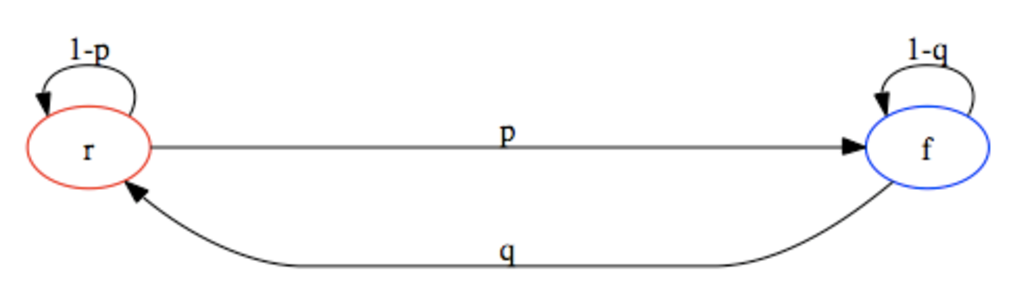
\includegraphics[width=6.5in]{figures/FlippantFreddyTransDiag}}
\end{figure}

Then Freddy's sequence of jumps $(X_0, X_1,\ldots)$ is a Markov chain on $\Xz$ with transition matrix:
\begin{equation}\label{E:FlippantFreddyP}
P 
= \bordermatrix{~ & r & f \cr 
r & P(r,r) & P(r,f)\cr 
f & P(f,r) & P(f,f) }
= \bordermatrix{~ & r & f \cr 
r & 1-p & p \cr
f & q & 1-q } \enspace .
\end{equation}
Suppose we first see Freddy in rollopia, i.e., $X_0=r$.  When he gets restless for the first time we know from the first row of $P$ that he will leave to flippopia with probability $p$ and stay with probability $1-p$, i.e.,
\begin{equation}\label{E:Freddy1Step}
\p(X_1=f | X_0=r) = p, \quad \p(X_1=r | X_0=r) = 1-p \enspace .
\end{equation}
What happens when he is restless for the second time?  By considering the two possibilities for $X_1$, Definition of conditional probability and the Markov property, we see that,
\begin{eqnarray}
\p(X_2 = f | X_0 = r) 
&=& \p(X_2=f, X_1=f | X_0=r) + \p(X_2=f, X_1=r | X_0=r) \notag \\
&=& \frac{\p(X_2=f, X_1=f , X_0=r)}{\p(X_0=r)} + \frac{\p(X_2=f, X_1=r , X_0=r)}{\p(X_0=r)} \notag \\
&=& \p(X_2=f | X_1=f , X_0=r)\frac{\p(X_1=f , X_0=r)}{\p(X_0=r)} \notag \\
&& \qquad + \p(X_2=f | X_1=r , X_0=r) \frac{\p(X_1=r , X_0=r)}{\p(X_0=r)} \notag \\
%&=& \frac{\p(X_2=f | X_1=f , X_0=r)\p(X_1=f | X_0=r)\p(X_0=r)}{\p(X_0=r)} \\
%&& \qquad + \frac{\p(X_2=f | X_1=r , X_0=r) \p(X_1=r | X_0=r)\p(X_0=r)}{\p(X_0=r)} \\
&=&{\p(X_2=f | X_1=f , X_0=r)\p(X_1=f | X_0=r)} \notag \\
&& \qquad +{\p(X_2=f | X_1=r , X_0=r) \p(X_1=r | X_0=r)} \notag \\
&=& \p(X_2=f | X_1=f) \p(X_1=f | X_0=r) \notag \\
&& \qquad+ \p(X_2=f | X_1=r) \p(X_1=r | X_0=r) \notag \\
&=& P(f,f) P(r,f) + P(r,f) P(r,r) \notag \\
&=& (1-q) p + p (1-p) \label{E:Freddy2Stepa}
\end{eqnarray}
Similarly, 
\begin{equation} \label{E:Freddy2Stepb}
\p(X_2=r | X_0 =r) = P(f,r) P(r,f) + P(r,r) P(r,r) = q p + (1-p)(1-p)
\end{equation}
Instead of elaborate computations of the probabilities of being in a given state after Freddy's $t$-th restless moment, we can store the state probabilities at time $t$ in a row vector:
\[
\mu_t := \left(  \p(X_t = r | X_0 = r), \p(X_t=f | X_0=r) \right) \enspace ,
\]
Now, we can conveniently represent Freddy starting in rollopia by the {\bf initial distribution} $\mu_0 = (1,0)$ and obtain the 1-step {\bf state probability vector} in \eqref{E:Freddy1Step} from $\mu_1 = \mu_0 P$ and the 2-step state probabilities in \eqref{E:Freddy2Stepa} and \eqref{E:Freddy2Stepb} by $\mu_2 = \mu_1 P = \mu_0 P P = \mu_0 P^2$.  In general, multiplying $\mu_t$, the state probability vector at time $t$, by the transition matrix $P$ on the right updates the state probabilities by another step:
\[
\mu_{t} = \mu_{t-1} P \qquad \text{for all } t \geq 1 \enspace .
\]
And for any initial distribution $\mu_0$,
\[
\mu_{t} = \mu_0 P^t  \qquad \text{for all } t \geq 0 \enspace .
\]
This can be easily implemented in \Matlab as follows:
%\begin{VrbM}
%>> p=0.5; q=0.5; P = [1-p p; q 1-q] % assume a fair coin and a fair die
%P =
%    0.5000    0.5000
%    0.5000    0.5000
%
%>> mu0 = [1, 0] % inital state vector since Freddy started in rollopia
%mu0 =     1     0
%
%>> mu0*P^0    % intial state distribution at t=0 is just mu0
%ans =     1     0
%
%>> mu0*P^1    % state distribution at t=1
%ans =    0.5000    0.5000
%
%>> mu0*P^2    % state distribution at t=2
%ans =    0.5000    0.5000
%\end{VrbM}
%Thus for a fair coin and die we get equal probabilities of being in the two states right after the first jump.  Let us see what happens for an unfair coin and die:
\begin{VrbM}
>> p=0.85; q=0.35; P = [1-p p; q 1-q] % assume an unfair coin and an unfair die
P =
    0.1500    0.8500
    0.3500    0.6500
>> mu0 = [1, 0] % inital state vector since Freddy started in rollopia
mu0 =     1     0
>> mu0*P^0    % intial state distribution at t=0 is just mu0
ans =     1     0
>> mu0*P^1    % state distribution at t=1
ans =    0.1500    0.8500
>> mu0*P^2    % state distribution at t=2
ans =    0.3200    0.6800
>> mu0*P^3    % state distribution at t=3
ans =    0.2860    0.7140
\end{VrbM}
Now, let us compute and look at the probability of being in rollopia after having started there for three values of $p$ and $q$ according to the following script: 
\VrbMf[label=FlippantFreddyRollopiaProbs.m]{scripts/FlippantFreddyRollopiaProbs.m}

\begin{figure}[htpb]
\caption{The probability of being back in rollopia in $t$ time steps after having started there under transition matrix $P$ with (i) $p=q=0.5$ (blue line with asterisks), (ii) $p=0.85$, $q=0.35$ (black line with dots) and (iii) $p=0.15$, $q=0.95$ (red line with pluses).\label{F:FlippantFreddyRollopiaProbs}}
\centering   \makebox{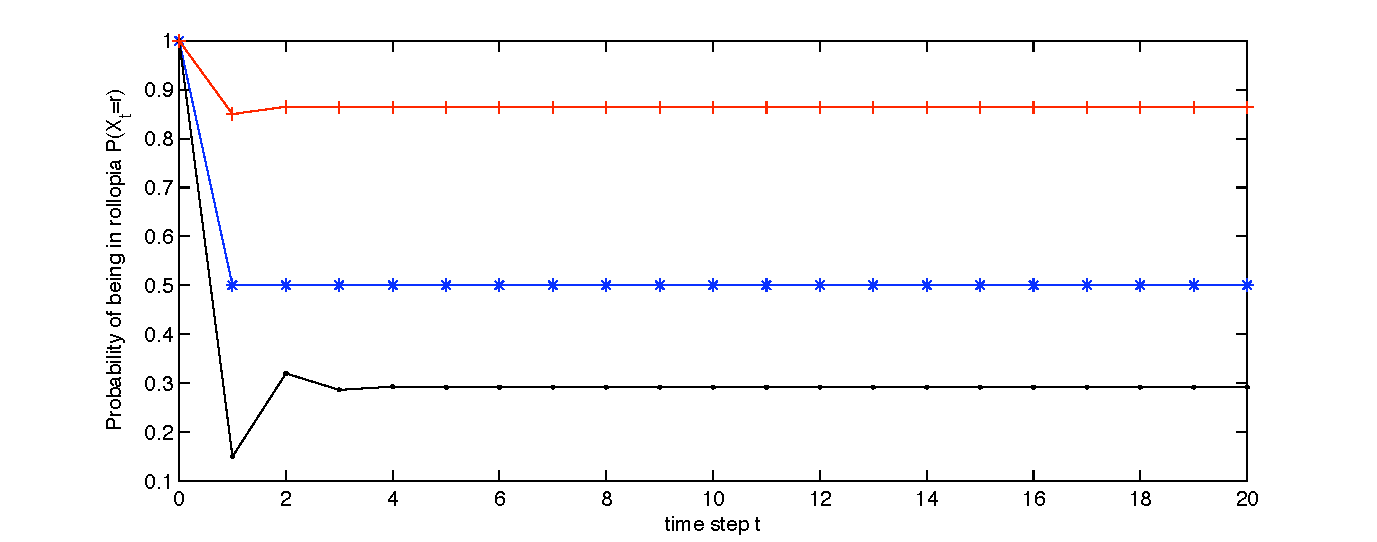
\includegraphics[width=6.5in]{figures/FlippantFreddyRollopiaProbs}}
\end{figure}

It is evident from \hyperref[F:FlippantFreddyRollopiaProbs]{Figure~\ref*{F:FlippantFreddyRollopiaProbs}} that as $t \to \infty$, $\mu_t$ approaches a distribution, say $\pi$, that depends on $p$ and $q$ in $P$.  Such a limit distribution is called the {\bf stationary distribution} and must satisfy the fixed point condition:
\[
\pi P = \pi \enspace ,
\]
that gives the solution:
\[
\pi(r) = \frac{q}{p+q}, \qquad \pi(f) = \frac{p}{p+q} \enspace .
\]
In \hyperref[F:FlippantFreddyRollopiaProbs]{Figure~\ref*{F:FlippantFreddyRollopiaProbs}} we see that $\p(X_t=r)$ approaches $\pi(r) = \frac{q}{p+q}$ for the three cases of $p$ and $q$:
\begin{align*}
\text{(i)}& \ p=0.50, q=0.50, & \p(X_t=r) & \to \pi(r) = \frac{q}{p+q} =  \frac{0.50}{0.50+0.50} = 0.5000,\\
\text{(ii)}& \  p=0.85, q=0.35, & \p(X_t=r) & \to \pi(r) = \frac{q}{p+q} =  \frac{0.35}{0.85+0.35} = 0.2917, \\
\text{(iii)}& \ p=0.15, q=0.95, & \p(X_t=r) & \to \pi(r) = \frac{q}{p+q} = \frac{0.95}{0.15+0.95} = 0.8636.
\end{align*}
\end{example}

Now let us generalise the lessons learned from \hyperref[EX:FlippantFreddy]{Example~\ref*{EX:FlippantFreddy}}.

\begin{prop}\label{P:FiniteMCProbsAtTimet}
For a finite Markov chain $\left(X_t\right)_{t \in \Zz_+}$ with state space $\Xz=\{s_1,s_2,\ldots,s_k\}$, initial distribution $$\mu_0 := \left( \mu_0(s_1), \mu_0(s_2), \ldots, \mu_0(s_k) \right),$$ where $\mu_0(s_i) = \p(X_0=s_i)$, and transition matrix $$P := \left(P(s_i,s_j)\right)_{(s_i,s_j)\in \Xz^2},$$ we have for any $t \in \Zz_+$ that the distribution at time $t$ given by:
$$\mu_t := \left( \mu_t(s_1), \mu_t(s_2), \ldots, \mu_t(s_k) \right),$$
where $\mu_t(s_i) = \p(X_t=s_i)$, satisfies:
\begin{equation}\label{E:mutismu0Pt}
\mu_t = \mu_0 P^t \enspace .
\end{equation}
\begin{proof}
We will prove this by induction on $\Z_+:=\{0,1,2,\ldots\}$.  First consider the case when $t=0$.  Since $P^0$ is the identity matrix $I$, we get the desired equality:
\[
\mu_0 P^0 = \mu_0 I = \mu_0 \enspace .
\]
Next consider the case when $t=1$.  We get for each $j \in \{1,2,\ldots,k\}$, that
\begin{align*}
\mu_1(s_j) &= \p(X_1 = s_j) = \sum_{i=1}^k \p(X_1=s_j,X_0=s_i)\\
&= \sum_{i=1}^k \p(X_1=s_j | X_0=s_i) \p(X_0=s_i) \\
&= \sum_{i=1}^k P(s_i,s_j) \mu_0(s_i)\\
&= (\mu_0 P)(s_j), \quad \text{the $j$-th entry of the row vector $(\mu_0 P)$} \enspace .
\end{align*}
Hence, $\mu_1=\mu_0 P$.  Now, we will fix $m$ and suppose that \eqref{E:mutismu0Pt} holds for $t=m$ and prove that \eqref{E:mutismu0Pt} also holds for $t=m+1$.  
For each $j \in \{1,2,\ldots,k\}$, we get
\begin{align*}
\mu_{m+1}(s_j) &= \p(X_{m+1} = s_j) = \sum_{i=1}^k \p(X_{m+1}=s_j,X_m=s_i)\\
&= \sum_{i=1}^k \p(X_{m+1}=s_j | X_m=s_i) \p(X_m=s_i) \\
&= \sum_{i=1}^k P(s_i,s_j) \mu_m(s_i)\\
&= (\mu_m P)(s_j), \quad \text{the $j$-th entry of the row vector $(\mu_m P)$} \enspace .
\end{align*}
Hence, $\mu_{m+1}=\mu_m P$.  But $\mu_{m}=\mu_0 P^m$ by the induction hypothesis, and therefore:
\[
\mu_{m+1} = \mu_m P = \mu_0 P^m P = \mu_0 P^{m+1} \enspace .
\]
Thus by the principle of mathematical induction we have proved the proposition.
\end{proof}
\end{prop}
Thus, multiplying a row vector $\mu_0$ by $P^t$ on the right takes you from current distribution over the state space to the distribution in $t$ steps of the chain.  

Since we will be interested in Markov chains on $\Xz =\{s_1,s_2,\ldots,s_k\}$ with the same transition matrix $P$ but different initial distributions, we introduce $\p_{\mu}$ and $\e_{\mu}$ for probabilities and expectations  given that the initial distribution is $\mu$, respectively.  When the initial distribution is concentrated at a single initial state $x$ given by:
$$\BB{1}_{\{x\}}(y) := \begin{cases} 1 & \text{if } y=x\\ 0 & \text{if } y \neq x \end{cases}$$ 
we represent it by $e_x$, the $1 \times k$ ortho-normal basis row vector with a $1$ in the $x$-th entry and a $0$ elsewhere.  
We simply write $\p_x$ for $\p_{\BB{1}_{\{x\}}}$ or $\p_{e_x}$ and $\e_x$ for $\e_{\BB{1}_{\{x\}}}$ or $\e_{e_x}$.  Thus, \hyperref[P:FiniteMCProbsAtTimet]{Proposition~\ref*{P:FiniteMCProbsAtTimet}} along with our new notations means that:
\[
\p_x (X_t = y)  = (e_x P^t)(y) = P^t(x,y) \enspace .
\]
In words, the probability of going to $y$ from $x$ in $t$ steps is given by the $(x,y)$-th entry of $P^t$, the {\bf $t$-step transition matrix}.  We refer to the $x$-th row and the $x$-th column of $P$ by $P(x,\cdot)$ and $P(\cdot,x)$, respectively.

Let the function $f(x): \Xz\to \Rz$ be represented by the column vector $f := (f(s_1),f(s_2),\ldots,f(s_k)) \in \Rz^{k \times 1}$.  Then the $x$-th entry of $P^t f$ is:
\[
P^t f(x) = \sum_{y} P^t(x,y) f(y) = \sum_{y} f(y) \p_x (X_t = y) = \e_x (f(X_t)) \enspace .
\] 
This is the expected value of $f$ under the distribution of states in $t$ steps given that we start at state $x$.  
Thus multiplying a column vector $f$ by $P^t$ from the left takes you from a function on the state space to its expected value in $t$ steps of the chain. 

%Let us look at some more examples of Markov chains.
\begin{example}[Dry-Wet Christchurch Weather]\label{EX:DryWetChain}
Consider a toy weather model for dry or wet days in Christchurch using a Markov chain with state space $\{d,w\}$.  Let the transition diagram in \hyperref[F:DryWetTransDiag]{Figure~\ref*{F:DryWetTransDiag}} give the transition matrix $P$ for our dry-wet Markov chain.  
\begin{figure}[htpb]
\caption{Transition Diagram of Dry and Wet Days in Christchurch.\label{F:DryWetTransDiag}}
\centering   \makebox{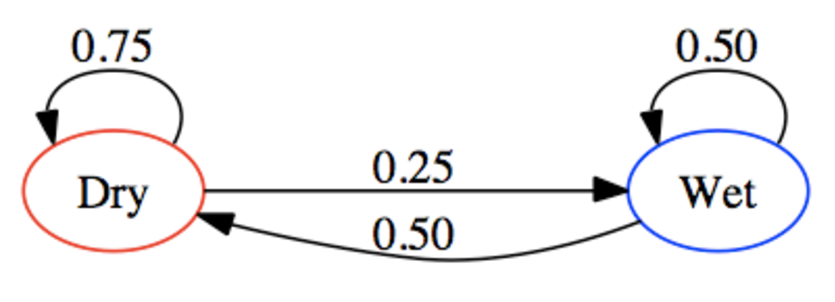
\includegraphics[width=3.5in]{figures/DryWetTransDiag}}
\end{figure}
Using \eqref{E:mutismu0Pt} we can find that the probability of being dry on the day after tomorrow is $0.625$ given that it is wet today as follows:
\begin{VrbM}
>> P=[0.75 0.25; 0.5 0.5] % Transition Probability Matrix
P =
    0.7500    0.2500
    0.5000    0.5000
>> mu0=[0 1] % it is wet today gives the initial distribution
mu0 =     0     1
>> mu0 * P^2 % the distribution in 2 days from today
ans =    0.6250    0.3750
\end{VrbM}
Suppose you sell \$100 of lemonade at a road-side stand on a hot day but only \$50 on a cold day.  Then we can compute your expected sales tomorrow if today is dry as follows:
\begin{VrbM}
>> P=[0.75 0.25; 0.5 0.5] % Transition Probability Matrix
P =
    0.7500    0.2500
    0.5000    0.5000
>> f = [100; 50] % sales of lemonade in dollars on a dry and wet day
f =
   100
    50
>> P*f % expected sales tomorrow
ans =
   87.5000
   75.0000 
>> mu0 = [1 0] % today is dry
mu0 =     1     0
>> mu0*P*f % expected sales tomorrow if today is dry
ans =   87.5000
\end{VrbM}
\end{example}

\begin{exercise}[Freddy discovers a gold coin]\label{EXR:FreddyGoldCoin}
Flippant Freddy of \hyperref[EX:FlippantFreddy]{Example~\ref*{EX:FlippantFreddy}} found a gold coin at the bottom of the pond.  Since this discovery he  jumps around differently in the enchanted pond.  He can be found now in one of three states: flipopia, rollopia and hydropia (when he dives into the pond). His state space is $\Xz=\{r,f,h\}$ now and his transition mechanism is as follows: If he rolls an odd number with his fair die in rollopia he will jump to flipopia but if he rolls an even number then he will stay in rollopia only if the outcome is $2$ otherwise he will dive into hydropia.  If the fair gold coin toss at the bottom of hydropia is Heads then Freddy will swim to flipopia otherwise he will remain in hydropia. Finally, if he is in flipopia he will remain there if the silver coin lands Heads otherwise he will jump to rollopia.

Make a Markov chain model of the new jumping mechanism adopted by Freddy.  Draw the transition diagram, produce the transition matrix $P$ and compute using \Matlab the probability that Freddy will be in hydropia after one, two, three, four and five jumps given that he starts in hydropia.
\end{exercise}

\begin{exercise}\label{Exr:NonMarkovProjection1}
Let $(X_t)_{t\in\Zz_+}$ be a Markov chain with state space $\{a,b,c\}$, initial distribution $\mu_0=(1/3,1/3,1/3)$ and transition matrix 
$$P = 
\bordermatrix{~ & a & b & c \cr
a & 0 & 1 & 0\cr
b & 0 & 0 & 1\cr
c & 1 & 0 & 0} \enspace .
$$
For each $t$, define $Y_t = \BB{1}_{\{b,c\}}(X_t)$.  Show that $(Y_t)_{t\in\Zz_+}$ is not a Markov chain.
\end{exercise}

\begin{exercise}\label{Exr:RegularSampledChainIsMarkov}
Let $(X_t)_{t\in\Zz_+}$ be a (homogeneous) Markov chain on $\Xz=\{s_1,s_2,\ldots,s_k\}$ with transition matrix $P$ and initial distribution $\mu_0$.  For a given $m \in \Nz$, let $(Y_t)_{t\in\Zz_+}$ be a stochastic sequence with $Y_t = X_{mt}$.  Show that $(Y_t)_{t\in\Zz_+}$ is a Markov chain with transition matrix $P^m$.  This establishes that Markov chains that are sampled at regular time steps are also Markov chains.
\end{exercise}


Until now our Markov chains have been {\bf  homogeneous} in time according to \hyperref[D:TimeHomFiniteMC]{Definition~\ref*{D:TimeHomFiniteMC}}, i.e., the transition matrix $P$ does not change with time.  We define inhomogeneous Markov chains that allow their transition matrices to possibly change with time.  Such Markov chains are more realistic as models in some situations and more flexible as algorithms in the sequel.

\begin{definition}[Inhomogeneous finite Markov chain]\label{D:TimeInhomFiniteMC}
Let $P_1,P_2,\ldots$ be a sequence of $k \times k$ stochastic matrices satisfying the conditions in \hyperref[E:StochasticMatrixConds]{Equation~\ref*{E:StochasticMatrixConds}}.  Then, the stochastic sequence $\left( X_t \right)_{t \in \Z_+} := (X_0,X_1,\ldots)$ with finite state space $\Xz := \{s_1,s_2,\ldots,s_k\}$ is called an inhomogeneous Markov chain with transition matrices $P_1,P_2,\ldots$, if for all pairs of states $(x,y) \in \Xz \times \Xz$, all integers $t \geq 1$, and all probable historical events $H_{t-1} := \bigcap_{n=0}^{t-1} \{ X_n = x_n \}$ with $\p\left(H_{t-1} \cap \{X_t = x\} \right) > 0$, the following {\bf Markov property} is satisfied: 
\begin{equation}\label{E:InHomFiniteMarkovProperty}
\p\left(X_{t+1} = y | H_{t-1} \cap \{X_t = x\} \right)=\p\left(X_{t+1} = y | X_t = x \right) =: P_{t+1}(x,y) \enspace .
\end{equation}
\end{definition}

\begin{prop}\label{P:FiniteInHomMCProbsAtTimet}
For a finite inhomogeneous Markov chain $\left(X_t\right)_{t \in \Zz_+}$ with state space $\Xz=\{s_1,s_2,\ldots,s_k\}$, initial distribution $$\mu_0 := \left( \mu_0(s_1), \mu_0(s_2), \ldots, \mu_0(s_k) \right),$$ where $\mu_0(s_i) = \p(X_0=s_i)$, and transition matrices 
$$\left(P_1,P_2,\ldots\right), \quad P_t := \left(P_t(s_i,s_j)\right)_{(s_i,s_j)\in \Xz\times \Xz}, \ t \in \{1,2,\ldots\}$$ we have for any $t \in \Zz_+$ that the distribution at time $t$ given by:
$$\mu_t := \left( \mu_t(s_1), \mu_t(s_2), \ldots, \mu_t(s_k) \right),$$
where $\mu_t(s_i) = \p(X_t=s_i)$, satisfies:
\begin{equation}\label{E:InhomMutismu0Pt}
\mu_t = \mu_0 P_1 P_2 \cdots P_t \enspace .
\end{equation}
\begin{proof}
Left as \hyperref[Exr:ProveInHomMultismu0Pt]{Exercise~\ref*{Exr:ProveInHomMultismu0Pt}}.
\end{proof}
\end{prop}

\begin{exercise}\label{Exr:ProveInHomMultismu0Pt}
Prove \hyperref[P:FiniteInHomMCProbsAtTimet]{Proposition~\ref*{P:FiniteInHomMCProbsAtTimet}} using induction as done for \hyperref[P:FiniteMCProbsAtTimet]{Proposition~\ref*{P:FiniteMCProbsAtTimet}}.
\end{exercise}


\begin{example}[a more sophisticated dry-wet chain]\label{EX:DryWetChainHotCold}
Let us make a more sophisticated version of the dry-wet chain of \hyperref[EX:DryWetChain]{Example~\ref*{EX:DryWetChain}} with state space $\{d,w\}$ .  In order to take some seasonality into account in our weather model for dry and wet days in Christchurch, let us have two transition matrices for hot and cold days:
\[
P_{\text{hot}} = 
\bordermatrix{~ & d & w \cr
d & 0.95 & 0.05 \cr
w & 0.75 & 0.25},
\qquad
P_{\text{cold}} = 
\bordermatrix{~ & d & w \cr
d & 0.65 & 0.35 \cr
w & 0.45 & 0.55} \enspace .
\]
We say that a day is hot if its  maximum temperature is more than $20^{\circ}$ Celsius, otherwise it is cold.  We use the transition matrix for today to obtain the state probabilities for tomorrow.  If today is dry and hot and tomorrow is supposed to be cold then what is the probability that the day after tomorrow will be wet?  We can use \eqref{E:InhomMutismu0Pt} to obtain the answer as $0.36$: 
\begin{VrbM}
>> Phot = [0.95 0.05; 0.75 0.25] % Transition Probability Matrix for hot day
Phot =
    0.9500    0.0500
    0.7500    0.2500
>> Pcold = [0.65 0.35; 0.45 0.55] % Transition Probability Matrix for cold day
Pcold =
    0.6500    0.3500
    0.4500    0.5500
>> mu0 = [1 0] % today is dry
mu0 =     1     0
>> mu1 = mu0 * Phot % distribution for tomorrow since today is hot
mu1 =    0.9500    0.0500
>> mu2 = mu1 * Pcold % distribution for day after tomorrow since tomorrow is supposed to be cold
mu2 =    0.6400    0.3600
>> mu2 = mu0 * Phot * Pcold % we can also get the distribution for day after tomorrow directly
mu2 =    0.6400    0.3600
\end{VrbM}
\end{example}

\begin{exercise}\label{Exr:DryWetChainHotCold}
For the Markov chain in \hyperref[EX:DryWetChainHotCold]{Example~\ref*{EX:DryWetChainHotCold}}  compute the probability that the day after tomorrow is wet if today is dry and hot but tomorrow is supposed to be cold.
\end{exercise}

\section{Random Mapping Representation and Simulation}\label{S:FiniteMCRMRandSim}

In order to simulate $(x_0,x_1,\ldots,x_n)$, a sequential realisation or sequence of states visited by a Markov chain, say the sequence of lily pads that Flippant Freddy visits on his jumps, we need a random mapping representation of a Markov chain and its computer implementation.  

\begin{definition}[Random mapping representation (RMR)]\label{D:RMR}
A {\bf random mapping representation} (RMR) of a transition matrix $P := \left(P(x,y)\right)_{(x,y)\in\Xz^2}$ is a function 
\begin{equation}\label{E:RMRrho}
\rho(x,w): \Xz \times \Wz \to \Xz \enspace ,
\end{equation}
along with the auxiliary $\Wz$-valued random variable $W$, satisfying
\begin{equation}\label{E:RMRProbrho}
\p \left( \{ \rho \left( x,W \right) = y  \} \right) = P(x,y), \quad \text{for each } (x,y) \in \Xz^2 \enspace .
\end{equation}
\end{definition}

\begin{prop}[Markov chain from RMR]\label{P:MCFromRMR}
If $W_1,W_2,\ldots \overset{IID}{\sim} W$, the auxiliary RV in  a RMR of a transition matrix $P := \left(P(x,y)\right)_{(x,y)\in\Xz^2}$, and  $X_0 \sim \mu_0$, then $\left(X_t\right)_{t\in\Zz_+}$ defined by
\[
X_t = \rho \left(X_{t-1},W_t\right), \quad \text{for all } t \geq 1
\]
is a Markov chain with transition matrix $P$ and initial distribution $\mu_0$ on state space $\Xz$.
\begin{proof}
Left as \hyperref[EXR:ProofofMCFromRMR]{Exercise~\ref*{EXR:ProofofMCFromRMR}}.
\end{proof}
\end{prop}

\begin{exercise}\label{EXR:ProofofMCFromRMR}
Do the proof of \hyperref[P:MCFromRMR]{Proposition~\ref*{P:MCFromRMR}} by using the necessary Definitions.
\end{exercise}


\begin{example}[An RMR for Flippant Freddy]\label{EX:RMRFreddy}
Reconsider the Markov chain of Flippant Freddy with fair dice and fair coin on state space $\Xz=\{r,f\}$ with transition matrix 
$$P=\bordermatrix{~ & r & f \cr
r & 1/2 & 1/2\cr
f & 1/2 &1/2}\enspace .$$
Let the auxiliary RV $W$ have sample space $\Wz=\{0,1\}$.  Then an RMR $\rho: \Xz \times \Wz \to \Xz$ for this $P$ is given by 
\[
\rho (x,w) : \{r,f\} \times \{0,1\} \to \{r,f\},
\quad \rho(r,0)=r, \quad \rho(r,1)=f, \quad \rho(f,0)=f,  \quad \rho(f,1)=r ,
\]
with $\p(W=0)=\p(W=1)=1/2$.  Now let us check that our $\rho$ and $W$ satisfy \hyperref[E:RMRProbrho]{Equation~\ref*{E:RMRProbrho}}:
\begin{eqnarray*}
\bordermatrix{~ & r & f \cr
r & \p \left( \{ \rho (r,W) = r \} \right) & \p \left( \{ \rho (r,W) = f \} \right) \cr
f & \p \left( \{ \rho (f,W) = r \} \right) & \p \left( \{ \rho (f,W) = f \} \right) }
&=&
\bordermatrix{~ & r & f \cr
r & \p \left( W=0 \right) & \p \left( W=1 \right) \cr
f & \p \left( W=1 \right) & \p \left( W=0 \right)} \\
&=&
\bordermatrix{~ & r & f \cr
r & 1/2 & 1/2\cr
f & 1/2 &1/2}
=
P \enspace .
\end{eqnarray*}
Thus, by \hyperref[P:MCFromRMR]{Proposition~\ref*{P:MCFromRMR}} we can obtain Freddy's Markov chain $\left(X_t\right)_{t\in \Zz_+}$ by initialising $X_0 \sim \mu_0=(1,0)$, i.e., setting $X_0=r$ since Freddy starts at $r$, and defining
\[
X_t = \rho(X_{t-1},W_t), \quad \text{for all } t \geq 1, \text{ where, } W_1,W_2,\ldots \overset{IID}{\sim} \bernoulli(1/2) \text{ RV} \enspace .
\]
In other words, we can simulate a sequence of states or lily pads visited by Freddy by merely doing independent $\bernoulli(1/2)$ trials and use the mapping $\rho$.  A \Matlab implementation of this RMR $\rho$ as a \Matlab function is:
\VrbMf[label=RMR1OfFairFreddy.m]{scripts/RMR1OfFairFreddy.m}
We can simulate one realisation of the first two states $(x_0,x_1)$ visited by $(X_0,X_1)$ as follows:
\begin{VrbM}
>> % set PRNG to be twister with seed 19731511
>> RandStream.setDefaultStream(RandStream('mt19937ar','seed',19731511));
>> x0 = 'r' % set x_0 = 'r'
x0 = r
>> w1 = floor( rand + 0.5 ) % a Bernoulli(0.5) trial
w1 =     0
>> x1 = RMR1OfFairFreddy(x0,w1) % x_1 = rho(x_0,w1) is the state at time t=1
x1 = r
\end{VrbM}
We can simulate one realisation of the first 10 states $(x_0,x_1,\ldots,x_9)$ visited by $(X_0,X_1,\ldots, X_9)$ using a for loop as follows:
\begin{VrbM}
>> % set PRNG to be twister with seed 19731511
>> RandStream.setDefaultStream(RandStream('mt19937ar','seed',19731511));
>> x0 = 'r' % set x_0 = 'r'
x0 = r
>> xt = x0; % current state x_t is x_0
>> Visited = x0; % initialise the variable Visited to hold the visited states
>> for t = 1:9 % start a for loop for t = 1,2,...,9
xt = RMR1OfFairFreddy(xt, floor(rand+0.5) ); % update the current state at t
Visited = strcat(Visited,',',xt); % store the visited state in string Visited
end
>> Visited % disclose the string of visited state separated by commas
Visited = r,r,f,f,r,r,f,f,f,r
\end{VrbM}
If we change the seed to some other number and repeat the code above, we will get another realisation of visits $(x_0,x_1,\ldots,x_9)$ of $(X_0,X_1,\ldots,X_9)$.  However, there are many distinct RMRs of the same transition matrix $P$.  For example, we can define a new RMR $\rho^\prime$ from our first RMR $\rho$ for $P$ by $\rho^\prime(x,w)=\rho(x,1-w)$.  The reader should check that $\rho^\prime$ also satisfies \hyperref[E:RMRProbrho]{Equation~\ref*{E:RMRProbrho}} with $W \sim Bernoulli(1/2)$. But note that even for the same seed and the same PRNG the sequence of states $(x_0,x_1,\ldots,x_9)$ visited by $(X_0,X_1,\ldots,X_9)$ under the new RMR $\rho^\prime$ is different from that of the original RMR $\rho$:
\begin{VrbM}
>> % set PRNG to be twister with seed 19731511
>> RandStream.setDefaultStream(RandStream('mt19937ar','seed',19731511));
>> x0 = 'r' % set x_0 = 'r'
x0 = r
>> xt = x0; % current state x_t is x_0
>> Visited = x0; % initialise the variable Visited to hold the visited states
>> for t = 1:9 % start a for loop for t = 1,2,...,9
xt = RMR1OfFairFreddy(xt, 1-floor(rand+0.5) ); % update the current state at t with new RMR rho'
Visited = strcat(Visited,',',xt); % store the visited state in string Visited
end
>> Visited % disclose the string of visited state separated by commas under new RMR rho'
Visited = r,f,f,r,r,f,f,r,f,f
\end{VrbM}	
\end{example}

\begin{prop}[Existence and non-uniqueness of RMR]
Every transition matrix $P$ on a finite state space $\Xz$ has a random mapping representation (RMR) that is not necessarily unique.
\begin{proof}
Let $\Xz = \{s_1,s_2,\ldots,s_k\}$ be sequentially accessible by $\psi(i)=s_i :  \{1,2,\ldots,k\} \to \Xz)$.   We will prove the proposition constructively via the inversion sampler for $\Xz$-valued family of $\psi$-transformed $\demoivre$ RVs.  Let the auxiliary RV $W$ be $\uniform(0,1)$ with $\Wz=[0,1]$ and let $\rho(x,w): \Xz \times \Wz \to \Xz$ be given by $F^{[-1]}(u;\theta_1,\theta_2,\ldots,\theta_k)$ of \hyperref[E:deMoivreInverseDF]{Equation~\ref*{E:deMoivreInverseDF}}, the inverse DF of the $\demoivre(\theta_1,\theta_2,\ldots,\theta_k)$ RV, as follows:
\[
\rho(x,w) = \psi \left( F^{[-1]}\left(w; P(x,s_1), P(x,s_2), \ldots, P(x,s_k) \right) \right), \quad \text{for each } x \in \Xz \enspace .
\]
Then, by construction, this $\rho$ is indeed an RMR of $P$ since
\[
\p \left( \{ \rho(x,W)=y \} \right) = P(x,y) \quad \text{for each } (x,y) \in \Xz^2 \enspace .
\]
Non-uniqueness is established by constructing another RMR for $P$ as $\rho^\prime(x,w) = \rho(x,1-w)$.
\end{proof}
\end{prop}

\begin{labwork}[Markov chain from $\{\demoivre(P(x,.))\}_{x\in\Xz}$ RVs]\label{LW:MCSimBydeMoivre}
Let us implement a function that will take a transition matrix $P$ as input and produce a sequence of $n$ states $(x_0,x_1,\ldots,x_{n-1})$ visited by the corresponding Markov chain $(X_0,X_1,\ldots, X_n)$ using the function in the following M-file.
\VrbMf[label=MCSimBydeMoivre.m]{scripts/MCSimBydeMoivre.m}
\end{labwork}

\begin{simulation}[Another simulation of Freddy's jumps]\label{SIM:FlippantFreddyByMCSimBydeMoivre}
Let us simulate a sequence of 10 jumps of Flippant Freddy with fair dice and coin by using the function {\tt MCSimBydeMoivre} defined in \hyperref[LW:MCSimBydeMoivre]{Labwork~\ref*{LW:MCSimBydeMoivre}} as follows:
\begin{VrbM}
>> % set PRNG to be twister with seed 19731511
>> RandStream.setDefaultStream(RandStream('mt19937ar','seed',19731511));
>> MCSimBydeMoivre(1,[0.5 0.5; 0.5 0.5], 10)
ans =     1     1     2     1     2     1     2     1     1     2
\end{VrbM}
Here we need to further transform the output by $\psi: \{1,2\} \to \{r,f\}$ with $\psi(1)=r$ and $\psi(2)=f$.
\end{simulation}

\begin{labwork}[Markov chain from $\{\demoivre(P(x,.))\}_{x\in\Xz}$ RVs by Recursion]\label{LW:MCSimBydeMoivreRecurse}
Let us implement a recursive function that will take a transition matrix $P$ as input and produce a sequence of $n$ states $(x_0,x_1,\ldots,x_{n-1})$ visited by the corresponding Markov chain $(X_0,X_1,\ldots, X_n)$ using the function in the following M-file.
\VrbMf[label=MCSimBydeMoivreRecurse.m]{scripts/MCSimBydeMoivreRecurse.m}
Now, let us compare this recursive function to the function {\tt MCSimBydeMoivre} defined in \hyperref[LW:MCSimBydeMoivre]{Labwork~\ref*{LW:MCSimBydeMoivre}} as follows:
\VrbMf[label=CompareMCSimBydeMoivreMethods.m]{scripts/CompareMCSimBydeMoivreMethods.m}
\begin{VrbM}
>> CompareMCSimBydeMoivreMethods
P =
    0.3333    0.6667
    0.2500    0.8000
initial =
     2
VisitByMethod1 =
     2     2     2     1     2     2     1     1     2     2     2     1
VisitByMethod2 =
     2     2     2     1     2     2     1     1     2     2     2     1
\end{VrbM}
Therefore, both methods produce the same output.  The recursive version of the function is more versatile and useful in the sequel.
\end{labwork}

\begin{simulation}\label{SIM:FreddyGoldCoinRMR}
Using the function {\tt MCSimBydeMoivre} of \hyperref[LW:MCSimBydeMoivre]{Labwork~\ref*{LW:MCSimBydeMoivre}} simulate twenty states visited by the Markov chain in \hyperref[EXR:FreddyGoldCoin]{Exercise~\ref*{EXR:FreddyGoldCoin}}.
\end{simulation}

\begin{simulation}[Drunkard's walk around the block]\label{SIM:DrunkardsWalkBlock}
Consider the Markov chain $\left(X_t\right)_{t \in \Zz_+}$ on $\Xz=\{0,1,2,3\}$ with initial distribution $\BB{1}_{\{3\}}(x)$ and transition matrix 
$$P = 
\bordermatrix{~ & 0 & 1 & 2 & 3 \cr 
0 & 0 & 1/2 & 0 & 1/2\cr
1 & 1/2 & 0 & 1/2 & 0\cr
2 & 0 & 1/2 & 0 & 1/2\cr
3 & 1/2 & 0 & 1/2 & 0 } \enspace .
$$
Draw the transition diagram for this Markov chain.  Do you see why this chain can be called the ``drunkard's walk around the block''? Using the function {\tt MCSimBydeMoivre} of \hyperref[LW:MCSimBydeMoivre]{Labwork~\ref*{LW:MCSimBydeMoivre}} simulate a sequence of ten states visited by the drunkard (don't forget to subtract $1$ from the output of {\tt MCSimBydeMoivre} since $\psi(i)=i-1$ here). 
\end{simulation}

There are many distinct and interesting RMRs of any given transition matrix $P$ beyond that constructed in the proof above.  Good RMRs will typically simplify the simulation of a Markov chain.
Let us consider examples of Markov chains that can be simulated by simpler methods.

\begin{example}[Jukes \& Cantor Model of DNA mutation]  The ``blueprint'' of organisms on earth are typically given by a long sequence of deoxyribonucleic acid or DNA.  A DNA sequence of length $n$ can be thought of as a string made up of $n$ alphabets from the set of four nucleotides $\{a,c,g,t\}$.  For example a DNA sequence of length $3$ is $agg$ and another is $act$.  When an organism goes through time to ``stay alive'' it has to copy its DNA.  This copying process is not perfect and mistakes or mutations are made.  We can look at a particular position of a DNA sequence and keep track of its mutations using a simple Markov chain due to Jukes and Cantor [Jukes TH and Cantor CR (1969) Evolution of protein molecules. In Munro HN, editor, Mammalian Protein Metabolism, pp. 21-132, Academic Press, New York.] with the following transition probability matrix:
\[
P = 
\bordermatrix{~ & a & c & g & t \cr
a & 0 & \frac{1}{3} & \frac{1}{3} & \frac{1}{3} \cr
c & \frac{1}{3} & 0 & \frac{1}{3} & \frac{1}{3} \cr
g & \frac{1}{3} & \frac{1}{3} & 0 & \frac{1}{3} \cr
t & \frac{1}{3}  & \frac{1}{3} & \frac{1}{3} & 0} \enspace .
\]
Suppose you initially observe the particular position of a DNA sequence at state $c$ and want to simulate a sequence of states  visited due to mutation under this Markov chain model.   We can achieve this by improvising the inversion sampler for the equi-probable $\demoivre(1/3,1/3,1/3)$ RV (\hyperref[A:SimdeMoivreEqui]{Algorithm~\ref*{A:SimdeMoivreEqui}}) in the following RMR:
\[
\rho(x,U): \{a,c,g,t\} \times [0,1] \to \{a,c,g,t\}, \quad
\rho(x,U) = \psi_x \left( \lceil 3 U \rceil \right), \quad 
U \sim \uniform(0,1) \enspace ,
\] 
with any fixed bijection $\psi_x(i) : \{1,2,3\} \to  \{a,c,g,t\} \setminus \{x\}$ for each $x \in \{a,c,g,t\}$.  
Then we can produce a sequence of visited states as follows:
\[
X_0 \gets c, \quad X_i \gets \rho\left( X_{i-1}, U_i \right), \quad i=1,2,\ldots \enspace .
\]
\end{example}

\begin{example}[Six Lounges]\label{EX:SixLounges}  Suppose there are six lounges with  doors that allow you to go only in one direction.  These lounges are labelled by $1$, $2$, $3$, $4$, $5$ and $6$ and form our state space $\Xz$ with one-way-doors as shown in \hyperref[F:SixLounges]{Figure~\ref*{F:SixLounges}}.  
\begin{figure}[htbp]
\caption{Transition diagram over six lounges (without edge probabilities).\label{F:SixLounges}}
\centering \mbox{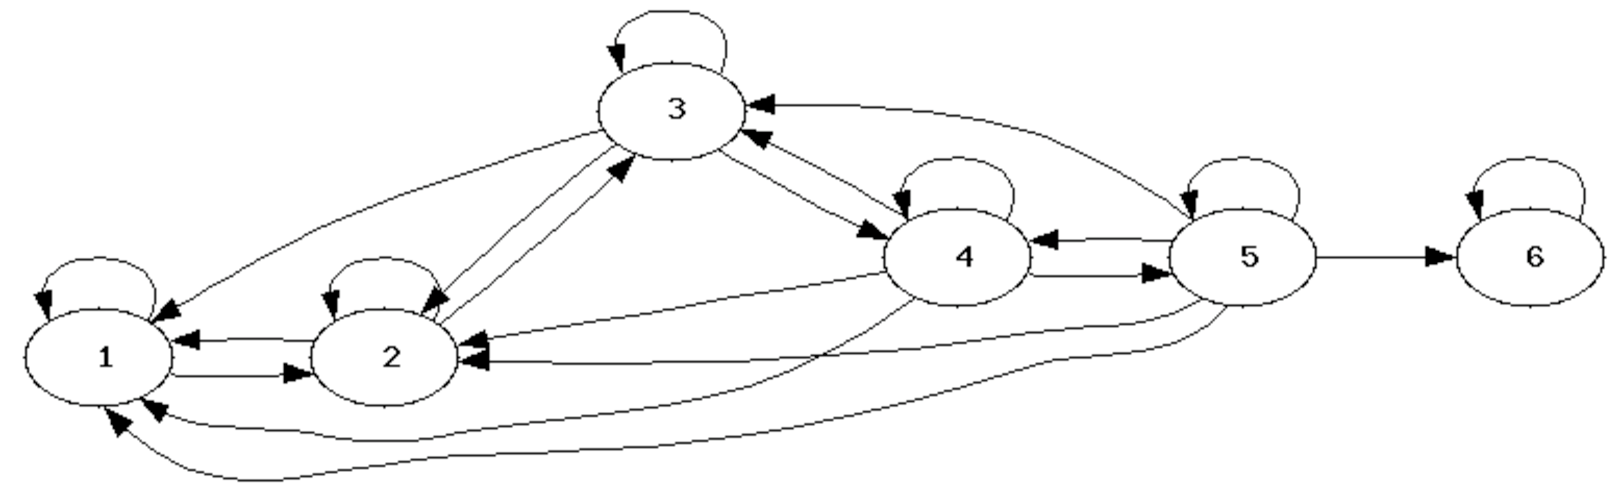
\includegraphics[width=4.5in]{figures/SixLounges}} 
\end{figure}
Every hour an alarm rings and it can be heard in all six lounges.  In each lounge $i \in \{1,2,3,4,5\}$ there is a fair $i$-sided polyhedral cylinder whose $i$ faces are marked with lounge numbers $1,2,\ldots,i$ but in lounge $6$ there is a hexagonal cylinder with all six faces marked by $6$.  Suppose you start from lounge number $1$.  When the hourly alarm rings you toss the ployhedral cylinder in the current lounge over the floor.  When the cylinder comes to rest, you note the number on the face that touches the floor and go to the lounge labelled by this number.  
This scheme of lounge hopping can be formalised as a Markov chain starting at lounge number $1$ and evolving according to the  transition matrix $P$:
$$P = 
\bordermatrix{ ~ & 1 & 2 & 3 &  4 & 5 & 6 \cr 
1 & \frac{1}{2} & \frac{1}{2} & 0 & 0 & 0 & 0 \cr
2 & \frac{1}{3} & \frac{1}{3} & \frac{1}{3} & 0 & 0 & 0 \cr
3 & \frac{1}{4} & \frac{1}{4} & \frac{1}{4} & \frac{1}{4} & 0 & 0 \cr
4 & \frac{1}{5} & \frac{1}{5} & \frac{1}{5} & \frac{1}{5} & \frac{1}{5} & 0 \cr
5 & \frac{1}{6} & \frac{1}{6} & \frac{1}{6} & \frac{1}{6} & \frac{1}{6} & \frac{1}{6} \cr
6 & 0 & 0 & 0 & 0 & 0 & 1 } \enspace .
$$
The inversion samplers for the family of equi-probable $\{\demoivre(1/i,1/i,\ldots,1/i)\}_{i \in \{1,2,\ldots,5\}}$ RVs (\hyperref[A:SimdeMoivreEqui]{Algorithm~\ref*{A:SimdeMoivreEqui}}) and the $\pointmass(6)$ RV (\hyperref[SIM:PointMass]{Simulation~\ref*{SIM:PointMass}}) can be combined in the random mapping representation:
$$
 \rho(i,U): \Xz \times [0,1] \to \Xz, \quad \rho(i,U) = \lceil i U \rceil \, \BB{1}_{\{1,2,3,4,5\}} (i) + 6 \, \BB{1}_{\{6\}}(i), \quad U \sim \uniform(0,1) \enspace ,$$
in order to simulate a sequence of states from this markov chain as follows:
\begin{equation}\label{E:SimulateSixLounges}
X_0 \gets 1, \quad X_i \gets \rho(X_{i-1},U_i), \quad i=1,2,\ldots \enspace .
\end{equation}
\end{example}

\begin{simulation}[Trapped in lounge $6$]\label{SIM:TrappedinLounge6}
Implement the Algorithm described in \hyperref[E:SimulateSixLounges]{Equation~\ref*{E:SimulateSixLounges}} in a \Matlab program to simulate the first ten states visited by the Markov chain in \hyperref[EX:SixLounges]{Example~\ref*{EX:SixLounges}}.  Recall the ``Hotel California'' character of  lounge $6$ -- {\em  you can check out anytime you like, but you can never leave}!  Repeat this simulation $1000$ times and find the fraction of times your are not trapped in lounge $6$ by the  tenth time step. 
\end{simulation}

\begin{exercise}[Drunkard's walk around a polygonal block with $k$ corners]\label{EXR:DrunkardWalkOnKGon}
Can you think of another way to simulate the ``drunkard's walk around a polygonal block with $k$ corners'' labelled by $0,1,\ldots, k-1$ that is more efficient than using the {\tt MCSimBydeMoivre} function which  relies on the {\tt SimdeMoivreOnce} function that implements \hyperref[A:SimdeMoivre]{Algorithm~\ref*{A:SimdeMoivre}} with an average-case efficiency that is linear in $k$?\\  {\scriptsize Hint: think of the drunkard tossing a fair coin to make his decision of where to go next from each corner and arithmetic mod $k$.}
\end{exercise}

\section{Irreducibility and Aperiodicity}\label{S:IrredAperiod}
The utility of our mathematical constructions with Markov chains depends on a delicate balance between generality and specificity.  We introduce two specific conditions called irreducibility and aperiodicity that make Markov chains more useful to model real-word phenomena.


\begin{definition}[Communication between states]\label{D:Communication} Let $(X_t)_{t\in\Zz_+}$ be a homogeneous Markov chain with transition matrix $P$ on state space $\Xz:=\{s_1,s_2,\ldots,s_k\}$.  
We say that a state $s_i$ {\bf communicates} with a state $s_j$ and write $s_i \rightarrow s_j$ or $s_j \leftarrow s_i$ if there exists an $\eta(s_i,s_j) \in \Nz$ such that:
\[
\p \left( X_{t+\eta(s_i,s_j)} = s_j | X_t = s_i \right) = P^{\eta(s_i,s_j)} (s_i, s_j) > 0 \enspace .
\] 
In words, $s_i$ communicates with $s_j$ if you can eventually reach $s_j$ from $s_i$.  If $P^{\eta} (s_i, s_j)=0$ for every $\eta \in \Nz$ then we say that $s_i$ {\bf does not communicate} with $s_j$ and write $s_i  \nrightarrow s_j$ or $s_j  \nleftarrow s_i$.

We say that two states $s_i$ and $s_j$ {\bf intercommunicate} and write $s_i \leftrightarrow s_j$ if $s_i \rightarrow s_j$ and $s_j \rightarrow s_i$.  In words, two states intercommunicate if you can eventually reach one from another and vice versa.  When $s_i$ and $s_j$ do not intercommunicate we write $s_i \nleftrightarrow s_j$.
\end{definition}

\begin{definition}[Irreducible]\label{D:Irreducible}
A homogeneous Markov chain $(X_t)_{t\in\Zz_+}$ with transition matrix $P$ on state space $\Xz:=\{s_1,s_2,\ldots,s_k\}$ is said to be {\bf irreducible} if $s_i \leftrightarrow s_j$ for each $(s_i,s_j) \in \Xz^2$.  Otherwise the chain is said to be {\bf reducible}.
\end{definition}

We have already seen examples of reducible and irreducible Markov chains.  For example, Flippant Freddy's family of Markov chains with the $(p,q)$-parametric family of transition matrices, $\{P_{(p,q)} : (p,q) \in [0,1]^2\}$, where each $P_{(p,q)}$ is given by \hyperref[E:FlippantFreddyP]{Equation~\ref*{E:FlippantFreddyP}}.  If $(p,q) \in (0,1)^2$, then the corresponding Markov chain is irreducible because we can go from rollopia to flippopia or vice versa in just one step with a positive probability.  Thus, the Markov chains with transition matrices in $\{P_{(p,q)} : (p,q) \in (0,1)^2\}$ are irreducible.  But if $p$ or $q$ take probability values at the boundary of $[0,1]$, i.e., $p \in \{0,1\}$ or $q \in \{0,1\}$ then we have to be more careful because we may  never get from at least one state to the other and the corresponding Markov chains may be reducible.   For instance, if $p=0$ or $q=0$ then we will be stuck in either rollopia or flippopia, respectively.  However, if $p=1$ and $q \neq 0$ or $q=1$ and $p \neq 0$ then we can get from each  state to the other.  Therefore,  only the transition matrices in $\left\{P_{(p,q)} : p \in \{0\} \text{ or } q \in \{0\}\right\}$ are reducible.

The simplest way to verify whether a Markov chain is irreducible is by looking at its transition diagram (without the positive edge probabilities) and checking that from each state there is a sequence of arrows leading to any other state.  For instance, from the transition diagram in \hyperref[F:SixLounges]{Figure~\ref*{F:SixLounges}} of the lounge-hopping Markov chain of \hyperref[EX:SixLounges]{Example~\ref*{EX:SixLounges}}, it is clear that if you start at state $6$ you cannot find any arrow going to any other state.  Therefore, the chain is reducible since $6 \nrightarrow i$ for any $i \in \{1,2,3,4,5\}$.

\begin{exercise}\label{EXR:ExsIrreducibleOrNot}
Revisit all the Markov chains we have considered up to now and determine whether they are reducible or irreducible by checking that from each state there is a sequence of arrows leading to any other state in their transition graphs.
\end{exercise}

\begin{definition}[Return times and period]
Let $\Tz(x) := \{t \in \Nz : P^t(x,x)>0\}$ be the set of {\bf possible return times} to the starting state $x$.  The {\bf period} of state $x$ is defined to be $\gcd(\Tz(x))$, the greatest common divisor of $\Tz(x)$.  When the period of a state $x$ is $1$, i.e., $\gcd(\Tz(x))=1$, then $x$ is said to be an {\bf aperiodic state}.
\end{definition}

\begin{prop}
If the Markov chain $(X_t)_{t\in\Zz_+}$ with transition matrix $P$ on state space $\Xz$ is irreducible then $\gcd(\Tz(x)) = \gcd(\Tz(y))$ for any $(x,y) \in \Xz^2$.
\begin{proof}
Fix any pair of states $(x,y) \in \Xz^2$.  Since, $P$ is irreducible, $x \leftrightarrow y$ and therefore there exists natural numbers $\eta(x,y)$ and $\eta(y,x)$ such that $P^{\eta(x,y)}(x,y)>0$ and $P^{\eta(y,x)}(y,x)>0$.  Let $\eta' = \eta(x,y)+\eta(y,x)$ and observe that $\eta' \in \Tz(x) \cap \Tz(y)$, $\Tz(x) \subset \Tz(y) - \eta' := \{t-\eta' : t \in \Tz(y)\}$ and $\gcd(\Tz(y))$ divides all elements in $\Tz(x)$.  Thus, $\gcd(\Tz(y)) \leq \gcd(\Tz(x))$.  By a similar argument we can also conclude that $\gcd(\Tz(x)) \leq \gcd(\Tz(y))$.  Therefore $\gcd(\Tz(x))=\gcd(\Tz(y))$.
\end{proof}
\end{prop}

\begin{definition}[Aperiodic]
A Markov chain $(X_t)_{t\in\Zz_+}$ with transition matrix $P$ on state space $\Xz$ is said to be {aperiodic} if all of its states are aperiodic, i.e., $\gcd(\Tz(x))=1$ for every $x \in \Xz$.  If a chain is not aperiodic, we call it {\bf periodic}.
\end{definition}

We have already seen example of irreducible Markov chains that  were either periodic or aperiodic.  For instance, Freddy's Markov chain with $(p,q) \in (0,1)^2$ is aperiodic since the period of either of its two states is given by $\gcd(\{1,2,3,\ldots\})=1$.  However, the Markov chain model for a drunkard's walk around a block over the state space $\{0,1,2,3\}$ (\hyperref[SIM:DrunkardsWalkBlock]{Simulation~\ref*{SIM:DrunkardsWalkBlock}}) is periodic because you can only return to the starting state in an even number of time steps and 
$$
\gcd(\Tz(0))=\gcd(\Tz(1))=\gcd(\Tz(2))=\gcd(\Tz(3))= \gcd \left( \{2,4,6,\ldots\} \right) =2 \neq 1 \enspace .
$$

\begin{exercise}\label{EXR:DrunkardsWalkOnKGonIrredAperiod}
Show that the Markov chain corresponding to a drunkard's walk around a polygonal block with $k$ corners is irreducible for any integer $k>1$.  Show that it is aperiodic only when $k$ is odd and has period $2$ when $k$ is even.
\end{exercise}

\begin{prop}\label{P:AdditionNonlattice} Let $A=\{a_1,a_2,\ldots\} \subset \Nz$ that satisfies the following two conditions:
\begin{enumerate}
\item $A$ is a {\bf nonlattice}, meaning that $\gcd(A)=1$ and
\item $A$ is closed undur addition, meaning that if $(a,a') \in A^2$ then $a+a' \in A$.
\end{enumerate}
Then there exists a positive integer $\eta < \infty$ such that $n \in A$ for all $n \geq \eta$.
\begin{proof}
See Proofs of Lemma 1.1, Lemma 1.2 and Theorem 1.1 in Appendix of {\em Pierre Br\'emaud, Markov Chains, Gibbs Fields, Monte Carlo Simulation, and Queues, Springer, 1999}.
\end{proof}
\end{prop}

\begin{prop}
If the Markov chain $(X_t)_{t\in\Zz_+}$ with transition matrix $P$ on state space $\Xz$ is irreducible and aperiodic then there is an integer $\tau$ such that $P^t(x,x)>0$ for all $t \geq \tau$ and all $x \in \Xz$.
\begin{proof}
TBD
\end{proof}
\end{prop}

\begin{prop}
If the Markov chain $(X_t)_{t\in\Zz_+}$ with transition matrix $P$ on state space $\Xz$ is irreducible and aperiodic then there is an integer $\tau$ such that $P^t(x,y)>0$ for all $t \geq \tau$ and all $(x,y) \in \Xz^2$.
\begin{proof}
TBD
\end{proof}
\end{prop}

\begin{exercise}[King's random walk on a chessboard]\label{EXR:KingRWChessBoard}
Consider the squares in the chessboard as the state space $\Xz = \{ 0,1,2,\ldots,7\}^2$ with a randomly walking black king, i.e., for each move from current state $(u,v) \in \Xz$ the king chooses one of his $k(u,v)$ possible moves uniformly at random.  
Is the Markov chain corresponding to the randomly walking black king on the chessboard irredicible and/or aperiodic?  
%Write a \Matlab script to simulate a sequence of $n$ states visited by the king if he started from $(0,0)$, the most south-west state on the chessboard.
\end{exercise}

\begin{exercise}[King's random walk on a chesstorus]\label{EXR:KingRWChessTorus}
We can obtain a chesstorus from a pliable chessboard by identifying the eastern edge with the western edge (roll the chessboard into a cylinder) and then identifying the northern edge with the southern edge (gluing the top and bottom end of the cylinder together by turning into a doughnut or torus).  Consider the squares in the chesstorus as the state space $\Xz = \{ 0,1,2,\ldots,7\}^2$ with a randomly walking black king, i.e., for each move from current state $(x,y) \in \Xz$ the king chooses one of his $8$ possible moves uniformly at random according to the scheme: $X_t \gets X_{t-1}+ W_t$, where $W_t$ is independent and identically distributed as follows:
\[ 
\p(W_t = w) = 
\begin{cases}
\frac{1}{8} & \text{if } w \in \left\{ (1,1), (1,0), (1,-1), (0,-1), (-1,-1), (-1,0), (-1,1), (0,1) \right\} , \\
0 & \text{ otherwise}.
\end{cases}
\]
Is the Markov chain corresponding to the randomly walking black king on the chesstorus irredicible and/or aperiodic?  Write a \Matlab script to simulate a sequence of $n$ states visited by the king if he started from $(0,0)$ on the chesstorus.
\end{exercise}

\section{Stationarity}\label{S:Stationarity}

We are interested in statements about a Markov chain that has been running for a long time.  
For any nontrivial Markov chain $(X_0,X_1,\ldots)$ the value of $X_t$ will keep fluctuating in the state space $\Xz$ as $t \to \infty$ and we cannot hope for convergence to a fixed point state $x^* \in \Xz$ or to a $k$-cycle of states $\{x_1,x_2,\ldots,x_k\} \subset \Xz$.  However, we can look one level up into the space of probability distributions over $\Xz$ that give the probability of the Markov chain visiting each state $x \in \Xz$ at time $t$, and hope that the distribution of $X_t$ over $\Xz$ settles down as $t \to \infty$.  The Markov chain convergence theorem indeed sattes that the distribution of $X_t$ over $\Xz$ settles down as $t \to \infty$, provided the Markov chain is irreducible and aperiodic.

\begin{definition}[Stationary distribution]
Let $\left( X_t \right)_{t \in \Zz_+}$ be a Markov chain with state space $\Xz=\{s_1,s_2,\ldots,s_k\}$ and transition matrix $P = \left( P(x,y) \right)_{(x,y) \in \Xz^2}$.  A row vector $$\pi = \left( \pi(s_1), \pi(s_2), \ldots, \pi(s_k) \right) \in \Rz^{1\times k}$$ is said to be a {\bf stationary distribution} for the Markov chain, if it satisfies the conditions of being:
\begin{enumerate}
\item {\em a probability distribution}: $\pi(x) \geq 0$ for each $x \in \Xz$ and $\sum_{x \in \Xz} \pi(x) = 1$, and
\item {\em a fixed point}: $\pi P = \pi$, i.e., $\sum_{x \in \Xz} \pi(x) P(x,y) = \pi(y)$ for each $y \in \Xz$.
\end{enumerate}
\end{definition}

\begin{definition}[Hitting times]
If a Markov chain $\left( X_t \right)_{t \in \Zz_+}$ with state space $\Xz=\{s_1,s_2,\ldots,s_k\}$ and transition matrix $P = \left( P(x,y) \right)_{(x,y) \in \Xz^2}$ starts at state $x$, then we can define the {\bf hitting time}
\[
T(x,y) = \min \{ t \geq 1: X_t = y \} \enspace .
\]
and let $T(x,y) = \min \{\} = \infty$ if the Markov chain never visits $y$ after having started from $x$.  Let the {\bf  mean hitting time} 
\[
\tau(x,y) := \e(T(x,y)) ,
\]
be the expected time taken to reach $y$ after having started at $x$.  Note that $\tau(x,x)$ is the {\bf mean return time} to state $x$.
\end{definition}

\begin{prop}[Hitting times of irreducible aperiodic Markov chains]  
If  $\left( X_t \right)_{t \in \Zz_+}$ is an irreducible aperiodic Markov chain with state space $\Xz=\{s_1,s_2,\ldots,s_k\}$, transition matrix $P = \left( P(x,y) \right)_{(x,y) \in \Xz^2}$ then for any pair of states ${(x,y) \in \Xz^2}$,
\[
\p\left( T(x,y) < \infty \right) = 1 \enspace ,
\]
and the mean hitting time is finite, i.e.,
\[
\tau(x,y) < \infty \enspace .
\]
\end{prop}

\begin{prop}[Existence of Stationary distribution]
For any irreducible and aperiodic Markov chain there exists at least one stationary distribution.
\begin{proof}
TBD
\end{proof}
\end{prop}

\begin{definition}[Total variation distance]\label{D:TotVarDist}
If $\nu_1:=\left(\nu_1(x)\right)_{x\in \Xz}$ and $\nu_2 := \left(\nu_2(x)\right)_{x\in \Xz}$ are elements of $\mathcal{P}(\Xz)$, the set of all probability distributions on $\Xz:=\{s_1,s_2,\ldots,s_k\}$, then we define the {\bf total variation distance} between $\nu_1$ and $\nu_2$ as
\begin{equation}\label{E:TotVarDist}
\dtv \left( \nu_1, \nu_2 \right) := \frac{1}{2} \sum_{x \Xz} \abs \left( \nu_1(x) - \nu_2(x) \right), \quad \dtv : \mathcal{P}(\Xz) \times \mathcal{P}(\Xz)  \to [0,1] \enspace .
\end{equation}
If $\nu_1, \nu_2, \ldots$ and $\nu$ are probability distributions on $\Xz$, then we say that $\nu_t$ {\bf converges in total variation} to $\nu$ as $n \to \infty$ and write $\nu_t  \overset{\mathsf{TV}}{\longrightarrow} \nu$, if
\[
\lim_{t \to \infty} \dtv \left( \nu_t, \nu \right) = 0 \enspace .
\]
Observe that if $\dtv(\nu_1,\nu_2)=0$ then $\nu_1=\nu_2$. The constant $1/2$ in \hyperref[E:TotVarDist]{Equation~\ref*{E:TotVarDist}} ensures that the range of $\dtv$ is in $[0,1]$.  If $\dtv(\nu_1,\nu_2)=1$ then $\nu_1$ and $\nu_2$ have disjoint  supports, i.e., we can partition $\Xz$ into $\Xz_1$ and $\Xz_2$, i.e., $\Xz=\Xz_1 \cup \Xz_2$ and $\Xz_1 \cap \Xz_2 = \emptyset$, such that $\sum_{x \in \Xz_1} \nu_1(x)=1$ and  $\sum_{x \in \Xz_2} \nu_2(x)=1$.  The total variation distance gets its name from the following natural interpretation:
\[
\dtv \left( \nu_1, \nu_2 \right) = \max_{A \subset \Xz} \abs \left( \nu_1(A) - \nu_2(A) \right) \enspace .
\]
This interpretation means that the total variation distance between $\nu_1$ and $\nu_2$ is the maximal difference in probabilities that the two distributions assign to any one event $A \in \sigma(\Xz) = 2^{\Xz}$. 
\end{definition}

In words, \hyperref[P:MCConvergence]{Proposition~\ref*{P:MCConvergence}} says that if you run the chain for a sufficiently long enough time $t$, then, regardless of the initial distribution $\mu_0$, the distribution at time $t$ will be close to the stationary distribution $\pi$.  This is referred to as the Markov chain {\bf approaching equilibrium} or {\bf stationarity} as $t \to \infty$.  

\begin{prop}[Markov chain convergence theorem]\label{P:MCConvergence}
Let $\left( X_t \right)_{t \in \Zz_+}$ be an irreducible aperiodic Markov chain with state space $\Xz=\{s_1,s_2,\ldots,s_k\}$, transition matrix $P = \left( P(x,y) \right)_{(x,y) \in \Xz^2}$ and initial distribution $\mu_0$.  Then for any distribution $\pi$ which is stationary for the transition matrix $P$, we have
\begin{equation}
\mu_t \overset{\mathsf{TV}}{\longrightarrow} \pi  \enspace .
\end{equation}
\begin{proof}
TBD
\end{proof}
\end{prop}

\begin{prop}[Uniqueness of stationary distribution]\label{P:UniqueStationaryDistrn}
Any irreducible aperiodic Markov chain has a unique stationary distribution.
\begin{proof}
TBD
\end{proof}
\end{prop}


\begin{exercise}\label{EXR:SixStatesWith3Blockof2}
Consider the Markov chain on $\{1,2,3,4,5,6\}$ with the following transition matrix:
\[
P = 
\bordermatrix{ ~ & 1 & 2 & 3 &  4 & 5 & 6 \cr 
1 & \frac{1}{2} & \frac{1}{2} & 0 & 0 & 0 & 0 \cr
2 & \frac{1}{2} & \frac{1}{2} & 0 & 0 & 0 & 0 \cr
3 & 0 & 0 &  \frac{1}{4} & \frac{3}{4} & 0 & 0  \cr
4 & 0 & 0 &  \frac{3}{4} & \frac{1}{4} & 0 & 0  \cr
5 & 0 & 0 &  0 & 0 & \frac{3}{4} & \frac{1}{4}  \cr
6 & 0 & 0 &  0 & 0 & \frac{1}{4} & \frac{3}{4}  } \enspace .
\]
Show that this chain is reducible and it has three stationary distributions:
\[
(1/2,1/2,0,0,0,0), \quad (0,0,1/2,1/2,0,0), \quad (0,0,0,0,1/2,1/2) \enspace .
\]
\end{exercise}

\begin{exercise}\label{EXR:ConvexCombof2StationaryDistrns}
If there are two stationary distributions $\pi$ and $\pi'$ then show that there is a infinite family of stationary distributions $\{\pi_p : p \in [0,1] \}$, called the convex combinations of $\pi$ and $\pi'$.
\end{exercise}

\begin{exercise}\label{EXR:ConvergengeinTVFailsforPeriodicDrunkardWalk}
Show that for a drunkard's walk chain started at state $0$ around a polygonal block with $k$ corners labelled $\{0,1,2,\ldots,k-1\}$, the state probability vector at time step $t$
\[
\mu_t \overset{\mathsf{TV}}{\longrightarrow} \pi   
\]
if and only if $k$ is odd.  Explain what happens to $\mu_t$ when $k$ is even.
\end{exercise}

\section{Reversibility}

We introduce another specific property called reversibility.  
This property will assist in conjuring Markov chains with a desired stationary distibution.

\begin{definition}[Reversible]\label{D:Reversible}
A probability distribution $\pi$ on $\Xz = \{s_1,s_2,\ldots,s_k\}$ is said to be a {\bf reversible distribution} for a Markov chain $\left(X_t\right)_{t\in \Zz}$ on $\Xz$ with transition matrix $P$ if for every pair of states $(x,y) \in \Xz^2$:
\begin{equation}\label{E:ReversibilityCondition}
\pi(x) P(x,y) = \pi(y) P(y,x) \enspace .
\end{equation}
A Markov chain that has a reversible distribution is said to be a reversible Markov chain.
\end{definition}

In words, $\pi(x) P(x,y) = \pi(y) P(y,x)$ says that if you start the chain at the reversible distribution $\pi$, i.e., $\mu_0 = \pi$, then the probability of going from $x$ to $y$ is the same as that of going from $y$ to $x$.

\begin{prop}[A reversible $\pi$ is a stationary $\pi$]\label{P:ReversibleIsStationary}
Let $\left(X_t\right)_{t \in \Zz_+}$ be a Markov chain on $\Xz = \{s_1,s_2,\ldots,s_k\}$ with transition matrix $P$.  
If $\pi$ is a reversible distribution for $\left(X_t\right)_{t \in \Zz_+}$ then $\pi$ is a stationary distribution for $\left(X_t\right)_{t \in \Zz_+}$.
\begin{proof}
Suppose $\pi$ is a reversible distribution for $\left(X_t\right)_{t \in \Zz_+}$ then $\pi$ is a probability distribution on $\Xz$ and $\pi(x) P(x,y) = \pi(y) P(y,x)$ for each $(x,y)\in \Xz^2$.  
We need to show that for any $y \in \Xz$ we have $$\pi(y)=\sum_{x\in\Xz}\pi(y) P(y,x) \enspace .$$ 
Fix a $y \in \Xz$,
\begin{eqnarray*}
LHS 
&=& \pi(y)= \pi(y) \, 1 = \pi(y) \, \sum_{x \in \Xz} P(y,x) \text{, since $P$ is a stochastic matrix} \\\\
&=& \sum_{x \in \Xz} \pi(y) P(y,x) = \sum_{x \in \Xz} \pi(x) P(x,y) \text{,  by reversibility} \\
&=& RHS \enspace .
\end{eqnarray*}
\end{proof}
\end{prop}


%\section{Classical Examples}
%\work
%\subsection{Random Walks on Graphs}

\begin{definition}[Graph]\label{D:Graph}
A {\bf Graph} $\Gz := (\Vz,\Ez)$ consists of a {\bf vertex set} $\Vz := \{v_1,v_2,\ldots,v_k\}$ together with an {\bf edge set} $\Ez := \{e_1,e_2,\ldots,e_l\}$.  Each edge connects two of the vertices in $\Vz$.  An edge $e_h$ connecting vertices $v_i$ and $v_j$ is denoted by $\langle v_i, v_j \rangle$.  Two vertices are {\bf neighbours} if they share an edge.  
The {\bf negihbourhood} of a vertex $v_i$ denoted by $\nbhd(v_i):=\left\{v_j : \langle v_i,v_j\rangle \in \Ez \right\}$ is the set of neighbouring vertices of $v_i$.  
The number of neighbours of a vertex $v_i$ in an undirected graph is called its {\bf degree} and is denoted by $\deg(v_i)$.  
Note that $\deg(v_i) = \# \nbhd(v_i)$.  
In a graph we only allow one edge per pair of vertices but in a {\bf multigraph} we allow more than one edge per pair of vertices.  
An edge can be {\bf directed} to preserve  the order of the pair of vertices they connect or they can be {\bf undirected}.  
An edge can be {\bf weighted} by being associated with a real number called its weight.  
We can represent a directed graph by its {\bf adjacency matrix} given by:
\[
A := \left( A(v_i,v_j) \right)_{(v_i,v_j) \in \Vz \times \Vz}, \quad 
A(v_i,v_j) = 
\begin{cases} 
1 & \text{if } \  \langle v_i, v_j \rangle \in \Ez \\
0 & \text{otherwise} \enspace .
\end{cases}
\]
Thus the adjacency matrix of an undirected graph is symmetric.  
In a directed graph, each vertex $v_i$ has {\bf in-edges} that come into it and {\bf out-edges} that go out of it.  
The number of in-edges and out-edges of $v_i$ is denoted by $\ideg(v_i)$ and $\odeg(v_i)$ respectively.  
Note that a transition diagram of a Markov chain is a weighted directed graph and is represented by the transition probability matrix.
\end{definition}

\begin{model}[Random Walk on an Undirected Graph]\label{M:RWGraph}
A random walk on an undirected graph $\Gz=(\Vz,\Ez)$ is a Markov chain with state space $\Vz:= \{v_1,v_2,\ldots,v_k\}$ and the following transition rules: if the chain is at vertex $v_i$ at time $t$ then it moves uniformly at random to one of the neighbours of $v_i$ at time $t+1$.  If $\deg(v_i)$ is the degree of $v_i$ then the transition probabilities of this Markov chain is
\[
P(v_i,v_j) = 
\begin{cases}
\frac{1}{\deg(v_i)} & \text{if $\langle v_i, v_j \rangle \in \Ez$}\\
0 & \text{otherwise} ,
\end{cases}
\]
\end{model}

\begin{prop}\label{P:RWUGpi}
The random walk on an undirected graph $\Gz=(\Vz,\Ez)$, with vertex set $\Vz:= \{v_1,v_2,\ldots,v_k\}$ and degree sum $d = \sum_{i=1}^k{\deg(v_i)}$ is a reversible Markov chain with the reversible distribution $\pi$ given by:
\[
\pi = \left( \frac{\deg(v_1)}{d}, \frac{\deg(v_2)}{d}, \ldots, \frac{\deg(v_k)}{d}  \right) \enspace .
\]
\begin{proof}
First note that $\pi$ is a probability distribution provided that $d > 0$.  
To show that $\pi$ is reversible we need to verify \hyperref[E:ReversibilityCondition]{Equation~\ref*{E:ReversibilityCondition}} for each $(v_i,v_j) \in \Vz^2$.  
Fix a pair of states $(v_i,v_j) \in \Vz^2$, then
\begin{eqnarray*}
\pi(v_i) P(v_i,v_j) = 
\begin{cases}
\frac{\deg(v_i)}{d}\frac{1}{\deg(v_i)}=\frac{1}{d}=\frac{\deg(v_j)}{d}\frac{1}{\deg(v_j)}=\pi(v_j) P(v_j,v_i) & \text{ if } \langle v_i, v_j \rangle \in \Ez\\
0 = \pi(v_j) P(v_j,v_i) & \text{ otherwise}.
\end{cases}
\end{eqnarray*} 
By \hyperref[P:ReversibleIsStationary]{Proposition~\ref*{P:ReversibleIsStationary}} $\pi$ is also the stationary distribution.
\end{proof}
\end{prop}

\begin{exercise}\label{EXR:DirectlyProveRWUGpi}
Prove \hyperref[P:RWUGpi]{Proposition~\ref*{P:RWUGpi}} by directly showing that $\pi P = \pi$, i.e., for each $v_i \in \Vz$, $\sum_{i=1}^k \pi(v_i) P(v_i, v_j) = \pi(v_j)$.
\end{exercise}

\begin{example}[Random Walk on a regular graph]\label{EX:RWRegGraph}
A graph $\Gz=(\Vz,\Ez)$ is called regular if every vertex in $\Vz=\{v_1,v_2,\ldots,v_k\}$ has the same degree $\delta$, i.e., $\deg(v_i)=\delta$ for every $v_i \in \Vz$.  
Consider the random walk on a regular graph with symmetric transition matrix 
\[
Q(v_i,v_j) = 
\begin{cases} 
\frac{1}{\delta} & \text{ if } \langle v_i,v_j \rangle \in \Ez \\
0 & \text{ otherwise}
\end{cases} \enspace .
\]
By \hyperref[P:RWUGpi]{Proposition~\ref*{P:RWUGpi}}, the stationary distribution of the random walk on $\Gz$ is the uniform distribution on $\Vz$ given by
\[
\pi 
= \left( \frac{\delta}{\delta \#\Vz }, \ldots , \frac{\delta}{\delta \#\Vz}  \right) 
= \left( \frac{1}{\#\Vz}, \ldots , \frac{1}{\#\Vz} \right) 
\enspace .
\]
\end{example}


\begin{example}[Triangulated Quadrangle]\label{EX:TriangulatedQuadrangle}
The random walk on the undirected graph 
$$\Gz=(\{1,2,3,4\}, \{\langle 1,2 \rangle, \langle 3,1 \rangle, \langle 2,3 \rangle, \langle 2,4 \rangle, \langle 4,3\rangle\})$$ depicted below with adjacency matrix $A$ is a Markov chain on $\{1,2,3,4\}$ with transition matrix $P$:
$$ 
A = 
\bordermatrix{~ & 1 & 2 & 3 & 4 \cr
1 & 0 & 1 & 1 & 0 \cr
2 & 1 & 0 & 1 & 1\cr
3 & 1 & 1 & 0 & 1\cr
4 & 0 & 1 & 1 & 0} ,
\quad
P = 
\bordermatrix{~ & 1 & 2 & 3 & 4 \cr
1 & 0 & \frac{1}{2} &  \frac{1}{2} & 0 \cr
2 & \frac{1}{3} & 0 &  \frac{1}{3} &  \frac{1}{3} \cr
3 & \frac{1}{3} &  \frac{1}{3} & 0 &  \frac{1}{3} \cr
4 & 0 &  \frac{1}{2} &  \frac{1}{2} & 0 } ,
\quad
\makebox{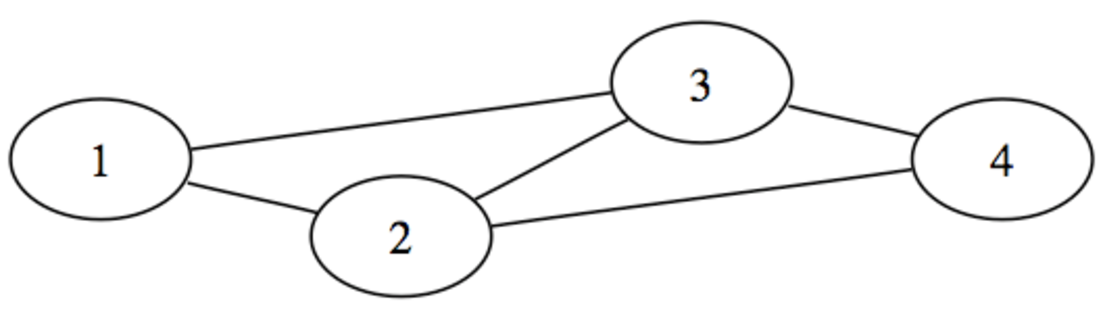
\includegraphics[width=2.5in]{figures/TriQuadrangle}}
\enspace .$$ 
By \hyperref[P:RWUGpi]{Proposition~\ref*{P:RWUGpi}}, the stationary distribution of the random walk on $\Gz$ is
\[
\pi = \left( \frac{\deg(v_1)}{d}, \frac{\deg(v_2)}{d}, \frac{\deg(v_3)}{d}, \frac{\deg(v_4)}{d} \right) 
= \left( \frac{2}{10}, \frac{3}{10}, \frac{3}{10}, \frac{2}{10} \right) \enspace .
\] 
\end{example}

\begin{exercise}\label{EXR:DrunkardAroundBlockFairReversible}
Show that the Drunkard's walk around the block from \hyperref[SIM:DrunkardsWalkBlock]{Simulation~\ref*{SIM:DrunkardsWalkBlock}} is a random walk on the undirected graph $\Gz=(\Vz,\Ez)$ with $\Vz=\{0,1,2,3\}$ and $\Ez=\{\langle 0,1 \rangle,\langle 1,2 \rangle,\langle 2,3 \rangle,\langle 0,3 \rangle \}$.  What is its reversible distribution?
\end{exercise}

\begin{example}[Drunkard's biased walk around the block]\label{SIM:DrunkardsBiasedWalkBlock}
Consider the Markov chain $\left(X_t\right)_{t \in \Zz_+}$ on $\Xz=\{0,1,2,3\}$ with initial distribution $\BB{1}_{\{3\}}(x)$ and transition matrix 
$$P = 
\bordermatrix{~ & 0 & 1 & 2 & 3 \cr 
0 & 0 & 1/3 & 0 & 2/3\cr
1 & 1/3 & 0 & 2/3 & 0\cr
2 & 0 & 1/3 & 0 & 2/3\cr
3 & 1/3 & 0 & 2/3 & 0 } \enspace .
$$
Draw the transition diagram for this Markov chain that corresponds to a drunkard who flips a biased coin to make his next move at each corner.  The stationary distribution is $\pi = (1/4,1/4,1/4,1/4)$ (verify $\pi P= \pi$).  

We will show that $\left(X_t\right)_{t \in \Zz_+}$ is not a reversible Markov chain.  
Sine $\left(X_t\right)_{t \in \Zz_+}$ is irreducible (aperiodicity is not necessary for uniqueness of $\pi$) $\pi$ is the unique stationary distribution.  
Due to \hyperref[P:ReversibleIsStationary]{Proposition~\ref*{P:ReversibleIsStationary}}, $\pi$ has to be a reversible distribution in order for $\left(X_t\right)_{t \in \Zz_+}$ to be a reversible Markov chain.  
But reversibility fails for $\pi$ since,
\[
\pi(0) P(0,1) = \frac{1}{4} \times \frac{1}{3} = \frac{1}{12} < \frac{1}{6} = \frac{1}{4} \times \frac{2}{3} = \pi(1)P(1,0) \enspace .
\]
\end{example}

\begin{exercise}\label{EXR:PiKingRWChessTorus}
Find the stationary distribution of the Markov chain in \hyperref[EXR:KingRWChessTorus]{Exercise~\ref*{EXR:KingRWChessTorus}}.
\end{exercise}

\begin{model}[Random Walk on a Directed Graph]\label{M:RWDGraph}
A random walk on a directed graph $\Gz=(\Vz,\Ez)$ is a Markov chain with state space $\Vz:= \{v_1,v_2,\ldots,v_k\}$ and transition matrix given by:
\[
P(v_i,v_j) = 
\begin{cases}
\frac{1}{\odeg(v_i)} & \text{if $\langle v_i, v_j \rangle \in \Ez$}\\
0 & \text{otherwise} ,
\end{cases}
\]
\end{model}

\begin{example}[Directed Triangulated Quadrangle]\label{EX:DirectedTriangulatedQuadrangle}
The random walk on the directed graph 
$$\Gz=(\{1,2,3,4\}, \{\langle 1,2 \rangle, \langle 3,1 \rangle, \langle 2,3 \rangle, \langle 2,4 \rangle, \langle 4,3\rangle\})$$ depicted below with adjacency matrix $A$ is a Markov chain on $\{1,2,3,4\}$ with transition matrix $P$:
$$ 
A = 
\bordermatrix{~ & 1 & 2 & 3 & 4 \cr
1 & 0 & 1 & 0 & 0 \cr
2 & 0 & 0 & 1 & 1 \cr
3 & 1 & 0 & 0 & 0 \cr
4 & 0 & 0 & 1 & 0},
\quad
P = 
\bordermatrix{~ & 1 & 2 & 3 & 4 \cr
1 & 0 & 1 & 0 & 0 \cr
2 & 0 & 0 & \frac{1}{2} & \frac{1}{2} \cr
3 & 1 & 0 & 0 & 0 \cr
4 & 0 & 0 & 1 & 0},
\quad
\makebox{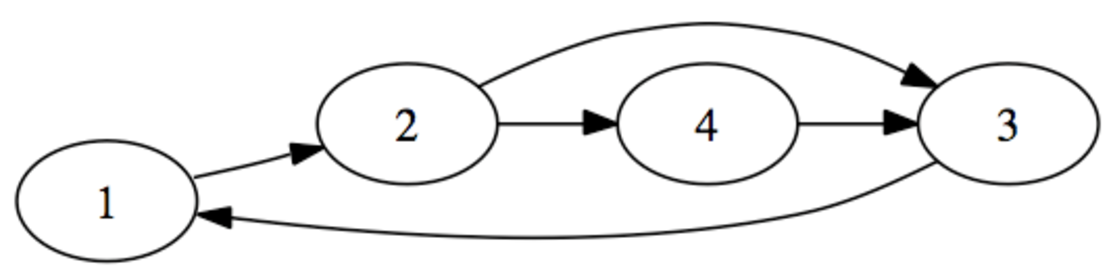
\includegraphics[width=2.5in]{figures/DirTriQuadrangle}}
\enspace .$$ 
\end{example}

\begin{exercise}\label{EXR:DirectedTriangulatedQuadrangleNoReversiblePi}
Show that the there is no reversible distibution for the Markov chain in \hyperref[EX:DirectedTriangulatedQuadrangle]{Example~\ref*{EX:DirectedTriangulatedQuadrangle}}. 
\end{exercise}

\begin{example}[Random surf on the word wide web]\label{EX:RandomSurferwww}
Consider the huge graph with vertices as webpages and hyper-links as undirected edges.  
Then \hyperref[M:RWGraph]{Model~\ref*{M:RWGraph}} gives a random walk on this graph.  
However if a page has no links to other pages, it becomes a sink and therefore terminates the random walk.  
Let us modify this random walk into a {\bf random surf} to avoid getting stuck.  
If the random surfer arrives at a sink page, she picks another page at random and continues surfing at random again.  
Google's PageRank formula uses a random surfer model who gets bored after several clicks and switches to a random page.  
The PageRank value of a page reflects the chance that the random surfer will land on that page by clicking on a link.  
The stationary distribution of the random surfer on the world wide web is a very successful model for ranking pages.
\end{example}

\begin{model}[Lazy Random Walk]
You can convert a random walk on an undirected graph $\Gz=(\Vz,\Ez)$ into a {\bf lazy random walk} on $\Gz$ by the following steps:
\begin{itemize}
\item Add loops to each vertex in $\Vz = \{v_1,v_2,\ldots,v_k\}$ to obtain a new set of edges $\Ez' = \Ez \cup \{\langle v_1,v_1 \rangle, \langle v_2,v_2 \rangle, \ldots, \langle v_k,v_k \rangle, \}$.
\item Construct the lazy graph $\Gz'=(\Vz,\Ez')$.
\item Do a random walk on the undirected graph $\Gz'$.
\end{itemize} 
The lazy random walk allows us to introduce aperiodicity quite easily.
\end{model}

\begin{exercise}[Lazy Random Walk on the Triangulated Quadrangle]\label{EXR:LazyWalkTriangulatedQuadrangle}
Consider the random walk of \hyperref[EX:TriangulatedQuadrangle]{Example~\ref*{EX:TriangulatedQuadrangle}} on the undirected graph 
$$\Gz=(\{1,2,3,4\}, \{\langle 1,2 \rangle, \langle 3,1 \rangle, \langle 2,3 \rangle, \langle 2,4 \rangle, \langle 4,3\rangle\}) \enspace .$$ 
Construct the lazy random walk on $\Gz$, obtain its transition probability matrix and state transition diagram.  
Show that the stationary distribution of this lazy random walk on $\Gz$ is
\[
\pi  
= \left( \frac{3}{14}, \frac{4}{14}, \frac{4}{14}, \frac{3}{14} \right) \enspace .
\] 
\end{exercise}

\begin{model}[Random Walks on Groups]
Under \work
\end{model}

\begin{model}[Birth-Death chains]
Under \work
\end{model}

%\subsection{Gambler's Ruin}
%\work
%\subsection{Cupon Collection}
%\work
%\subsection{Projection of random walk on hypercube to Ehrenfest's Urn}
%\work
%\work

%\section{State Classification}
%This Section is under \work.


% Estimation
\section{Metropolis-Hastings Markov chain}

\begin{definition}[Metropolis-Hastings Markov chain]\label{D:M-HChain}
If we are given an irreducible Markov chain $\left(Y_t\right)_{t\in \Zz_+}$ called the {\bf base chain} or the {\bf proposal chain} on a finite state space $\Xz = \{s_1,s_2,\ldots,s_k\}$ with transition probability matrix $Q = \left(Q(x,y)\right)_{(x,y)\in \Xz^2}$ and some probability distribution $\pi$ on $\Xz$ of interest that may only be known up to a normalizing constant as $\tilde{\pi}$, i.e., $\pi(x) = \left(\sum_{z \in \Xz}{\tilde{\pi}(z)}\right)^{-1} \tilde{\pi}(x)$ for each $x \in \Xz$, then we can construct a new Markov chain $\left(X_t\right)_{t\in \Zz_+}$ called the {\bf Metropolis-Hastings} chain on $\Xz$ with the following transition probabilities:
\begin{equation}\label{E:M-HPs}
P(x,y) = 
\begin{cases}
Q(x,y) a(x,y) & \text{ if } x \neq y\\
1 - \sum_{z \in \{z \in \Xz : z \neq x\}} Q(x,z) a(x,z) & \text{ if } x = y 
\end{cases} \enspace ,
\end{equation}
where the acceptance probability is
\begin{equation}\label{E:M-Ha}
a(x,y) := \min\left\{ 1, \frac{\pi(y)}{\pi(x)}\frac{Q(y,x)}{Q(x,y)} \right\} \enspace .
\end{equation}
Note that we only need to know $\pi$ up to ratios.  Thus, ${\pi(y)}/{\pi(x)}$ in $a(x,y)$ can be replaced by ${\tilde{\pi}(y)}/{\tilde{\pi}(x)}$ since
\[
\frac{\pi(y)}{\pi(x)}  
= \frac{\left(\sum_{z \in \Xz}{\tilde{\pi}(z)}\right)^{-1} \tilde{\pi}(y)}{\left(\sum_{z \in \Xz}{\tilde{\pi}(z)}\right)^{-1} \tilde{\pi}(x)} 
= \frac{\tilde{\pi}(y)}{\tilde{\pi}(x)} \enspace .
\]
\hyperref[A:MHSamplerFiniteMC]{Algorithm~\ref*{A:MHSamplerFiniteMC}} describes how to simulate samples from a Metropolis-Hastings Markov chain.  
\end{definition}

\begin{prop}[Stationarity of the Metropolis-Hastings chain]\label{P:M-HChainStationary}
The Metropolis-Hastings chain constructed according to \hyperref[D:M-HChain]{Definition~\ref*{D:M-HChain}} has $\pi$ as its stationary distribution.  
\begin{proof}
It suffices to show that $\pi$ is the reversible distribution for $\left(X_t\right)_{t\in \Z_+}$, i.e., for each $(x,y) \in \Xz^2$, $\pi(x)P(x,y) = \pi(y) P(y,x)$.  
Fix a pair $(x,y) \in \Xz^2$ and suppose $x\neq y$.  
Then,
\begin{eqnarray*}
\pi(x)P(x,y) 
&=& \pi(x) Q(x,y)a(x,y) \\
&=& \pi(x) Q(x,y) \min\left\{ 1, \frac{\pi(y)}{\pi(x)}\frac{Q(y,x)}{Q(x,y)} \right\} \\
&=& \min\left\{ \pi(x) Q(x,y), \pi(x) Q(x,y) \frac{\pi(y)}{\pi(x)}\frac{Q(y,x)}{Q(x,y)} \right\}\\
&=& \min\left\{ \pi(x) Q(x,y), \pi(y) Q(y,x) \right\}\\
&=& \min\left\{ \pi(y) Q(y,x), \pi(x) Q(x,y) \right\}\\
&=& \min\left\{ \pi(y) Q(y,x), \pi(y) Q(y,x) \frac{\pi(x)}{\pi(y)} \frac{Q(x,y)}{Q(y,x)} \right\}\\
&=& \pi(y) Q(y,x) \min\left\{ 1, \frac{\pi(x)}{\pi(y)} \frac{Q(x,y)}{Q(y,x)} \right\}\\
&=& \pi(y) P(y,x) \enspace .
\end{eqnarray*}
When $x=y$, reversibility is trivially satisfied since $\pi(x)P(x,y) = \pi(y) P(y,x)=\pi(x)P(x,x)$.
\end{proof}
\end{prop}

\begin{definition}\label{M:MetropolisChain}
If the base chain $\left(Y_t\right)_{t \in \Zz_+}$ in the Metropolis-Hastings Markov chain of \hyperref[D:M-HChain]{Definition~\ref*{D:M-HChain}} has a symmetric transition matrix $Q$ with $Q(x,y)=Q(y,x)$ for each $(x,y)\in \Xz^2$ then the acceptance probability in \hyperref[E:M-Ha]{Equation~\ref*{E:M-Ha}} simplifies to
\[
a(x,y) =  \min\left\{1, \frac{\pi(y)}{\pi(x)} \right\} \enspace ,
\]
and the corresponding Metropolis-Hastings chain $\left(X_t\right)_{t\in Zz_+}$ is called the {\bf Metropolis chain}.
\end{definition}

\begin{algorithm}%WORK rewrite
\caption{Metropolis-Hastings Markov chain}
\label{A:MHSamplerFiniteMC}
\begin{algorithmic}[1]
\STATE {
{\it input:} 
\begin{itemize}
\item[(1)] shape of a target density $\tilde{\pi}(x) = \left({\sum_{x \in \Xz} \tilde{\pi}(x)}\right) \pi(x)$,
\item[(2)] sampler for the base chain that can produce samples $y \sim Q(x,\cdot)$.
\end{itemize}
}
\STATE {\it output:} a sequence of samples $x_0,x_1, \ldots, x_n$ from the Metropolis-Hastings Markov chain $\left(X_t\right)_{t \in \Zz_+}$ with stationary distribution $\pi$
\STATE Choose initial state $x_0 \in \Xz$ according to $\mu_0$
\REPEAT
\STATE At iteration $t$,
\STATE Generate $y \sim Q(x_{t-1},\cdot)$ and $u \sim \uniform(0,1)$,
\STATE Compute {\it acceptance probability}
\[
a(x_{t-1},y)=\min\left\{1,\frac{\tilde{\pi}(y)}{\tilde{\pi}(x_{t-1})}\frac{Q(y,x_{t-1})}{Q(x_{t-1}),y} \right\},
\]
\STATE
{\bf If} $u \leq a(x_{t-1},y)$
{\bf then} $x_t \gets y$, 
{\bf else} $x_t \gets x_{t-1}$
\UNTIL desired number of samples $n$ are obtained from $\left(X_t\right)_{t \in \Zz_+}$
\end{algorithmic}
\end{algorithm}

Suppose you know neither the vertex set $\Vz$ nor the edge set $\Ez$ entirely for an undirected graph $\Gz=(\Vz,\Ez)$ but you are capable of walking locally on $\Gz$.  
In other words, if you are currently at vertex $x$ you are able to make a move to one of the neighbouring vertices of $x$.  
However, you do not know every single vertex in $\Vz$ or the entire set of edges $\Ez$ as an adjacency matrix for instance.  
Several real-world problems fall in this class.  
Some examples include the random surfer on www to rank web pages (\hyperref[EX:RandomSurferwww]{Example~\ref*{EX:RandomSurferwww}}), social network analyses in facebook or twitter, exact tests for contingency tables, etc.

\begin{model}[Metropolis-Hastings Random Walk on Graph]  
Let $\Gz=(\Vz,\Ez)$ be an undirected graph and let $\left(Y_t\right)_{t \in \Zz_+}$ with transition matrix $Q$ be an irreducible random walk on $\Gz$ and let $\pi$ be a probability distribution on $\Vz=\{v_1,v_2,\ldots,v_k\}$ that is known upto a normalizing constant as $\tilde{\pi}$.  
The {\bf Metropolis-Hastings random walk} on $\Gz$ is the Metropolis-Hasting Markov chain $\left(X_t\right)_{t\in \Zz_+}$ on $\Vz$ with base chain $\left(Y_t\right)_{t\in \Zz_+}$ and the following transition probabilities:
\[
P(x,y) = 
\begin{cases}
\frac{1}{\deg(v_i)}\min \left\{ 1, \frac{\tilde{\pi}(v_j)}{\tilde{\pi}(v_i)} \frac{\deg(v_i)}{\deg(v_j)} \right\} & \text{ if } \langle v_i,v_j \rangle \in \Ez \\
1 - \sum_{v_l \in \nbhd(v_i)} \left( \frac{1}{\deg(v_i)} \min \left\{ 1, \frac{\tilde{\pi}(v_l)}{\tilde{\pi}(v_i)} \frac{\deg(v_i)}{\deg(v_l)} \right\} \right) & \text{ if } v_i=v_j\\
0 & \text{ otherwise }
\end{cases} \enspace .
\]
By \hyperref[P:M-HChainStationary]{Proposition~\ref*{P:M-HChainStationary}}, $\left(X_t\right)_{t\in \Zz_+}$ has $\pi$ as its stationary distribution.
This Markov chain can be simulated as follows:
\begin{itemize}
\item Suppose $x_t = v_i$ at time $t$
\item Propose $v_j$ uniformly at random from $\nbhd(v_i)$
\item Sample $u$ from $\uniform(0,1)$
\item If $u < \min \{1, \pi(v_j)\deg(v_i)/\pi(v_i)\deg(v_j)\}$ then $x_{t+1}=v_j$ else $x_{t+1}=x_t$
\end{itemize}
\end{model}

\begin{model}[Metropolis chain on a regular graph]\label{M:MetropolisChainRWRegGraph}
Consider the random walk $\left(Y_t \right)_{t \in \Zz_+}$ on a regular graph $\Gz=(\Vz,\Ez)$ with $\deg(v_i)=\delta$ for every vertex $v_i \in \Vz=\{v_1,v_2,\ldots,v_k\}$ and the symmetric transition matrix 
\[
Q(v_i,v_j) = 
\begin{cases} 
\frac{1}{\delta} & \text{ if } \langle v_i,v_j \rangle \in \Ez \\
0 & \text{ otherwise}
\end{cases} \enspace .
\]
You can sample from a given distribution $\pi$ on $\Vz$ by constructing the Metropolis chain with stationary distribution $\pi$ from the base chain given by $\left(Y_t \right)_{t \in \Zz_+}$.
\end{model}

\begin{model}[sampling from a uniform distribution over an irregular graph]
A graph $\Gz=(\Vz,\Ez)$ that is not regular is said to be irregular.  Clearly, the stationary distribution of a random walk on $\Gz$ is not uniform.  
Suppose you want to sample uniformly from $\Vz$ according to $\pi(v_i)=(\#\Vz)^{-1}$ for each $v_i \in \Vz$.  
We can accomplish this by constructing a Metropolis-Hastings Markov chain with the random walk on $\Gz$ as the base chain and the following transition probabilities:
\[
P(v_i,v_j) = 
\begin{cases}
\frac{1}{\deg(v_i)}\min \left\{ 1, \frac{\deg(v_i)}{\deg(v_j)} \right\} & \text{ if } \langle v_i,v_j \rangle \in \Ez \\
1 - \sum_{v_l \in \nbhd(v_i)} \left( \frac{1}{\deg(v_i)} \min \left\{ 1, \frac{\deg(v_i)}{\deg(v_l)} \right\} \right) & \text{ if } v_i=v_j\\
0 & \text{ otherwise }
\end{cases} \enspace .
\]
Thus the Metropolis-Hastings walk on $\Gz$ is biased against visiting higher degree vertices and thereby samples unifromly from $\Vz$ at stationarity.
\end{model}

\begin{example}[Stochastic Optimization]
Lef $f: \Vz \to \Rz$ and $\Gz=(\Vz,\Ez)$ be an undirected graph.  Let the global maximum be
\[
f^* := \max_{y \in \Vz} f(y) \enspace ,
\]
and the set of maximizers of $f$ be
\[
\Vz^* := \argmax_{x \in \Vz} f(x) = \{ x \in \Vz : f(x) = f^* \} \enspace .
\]
In many problems such as maximum likelihood estimation, minimizing a cost function by maximizing its negative, etc, one is interested in $\Vz^* \subset \Vz$.  
This global maximization problem is difficult when $\# \Vz$ is huge.  
A deterministic hill-climbing or gradient ascent algorithm that iteratively moves from the current state $v_i$ to a neighbouring state $v_j$ if $f(v_j) > f(v_i)$ can easily get trapped in a local peak of $f$ and thereby miss the global peak attained by elements in $\Vz^*$.

\begin{figure}[htpb]
\caption{Stochatic Optimization with Metropolis chain.\label{F:StochasticOptimMetropolisChain}}
\centering   \makebox{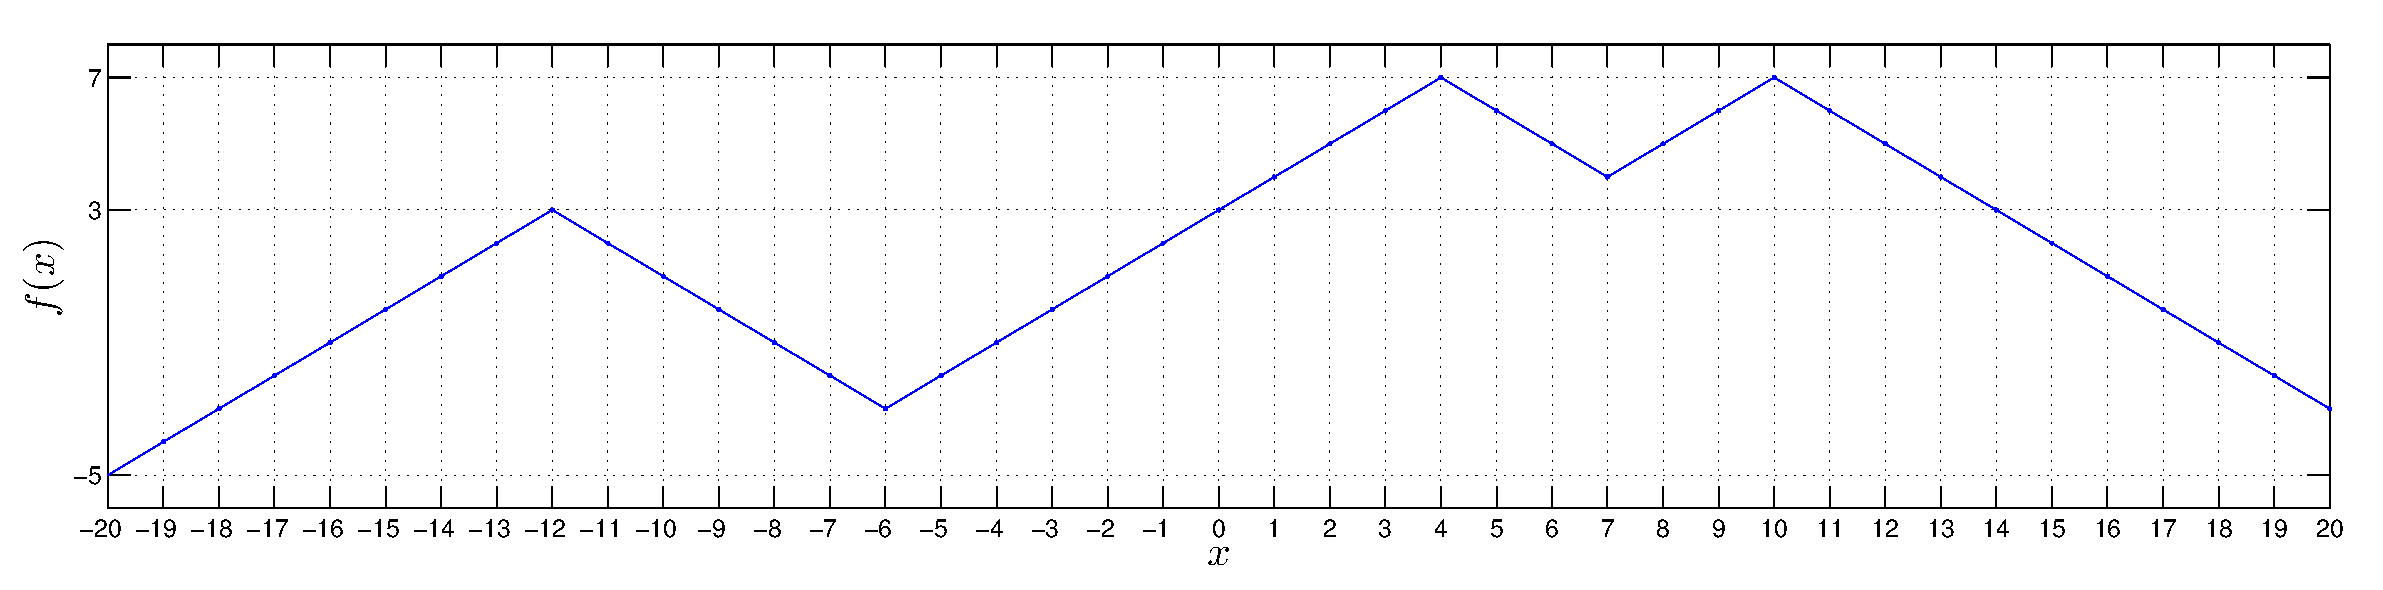
\includegraphics[width=6.5in]{figures/StochasticOptimMetropolisChain}}
\end{figure}
For example consider the global maximization problem shown in \hyperref[F:StochasticOptimMetropolisChain]{Figure~\ref*{F:StochasticOptimMetropolisChain}} with 
$$ f^* = 7 \text{ and } \Vz^* = \{4,10\} \subset \Vz = \{-20,-19,\ldots,19,20\} \enspace . $$
The deterministic hill-climbing algorithm will clearly miss $\Vz^*$ and terminate at the local maximum of $3$ at $-12$ if initialised at any element in $\{-20,-19,\ldots,-8,-7\}$.  
Also, this algorithm will not find both elements in $\Vz^*$ even when initialised more appropriately.

We will construct a Markov chain to solve this global maximization problem.  
For a fixed parameter $\lambda \in \Rz_{>0}$, let 
$$\pi_{\lambda}(x) = \frac{\lambda^{f(x)}}{\sum_{z \in \Vz} \lambda^{f(z)}} \enspace .$$
Since $\pi_{\lambda}(x)$ is increasing in $f(x)$, $\pi_{\lambda}(x)$ favours vertices with large $f(x)$.    
First form a graph $\Gz=(\Vz,\Ez)$ by adding edges between the vertices in $\Vz$ so that you can get from any vertex to any other vertex in $\Vz$ by following a sequence of edges in $\Ez$.  
Now using the random walk on $\Gz$ as the base chain let us construct a Metropolis-Hastings chain $\left(X_t\right)_{t \in \Zz_+}$ on $\Gz$ with $\pi_{\lambda}$ on $\Vz$ as its stationary distribution.  

For simplicity, let us suppose that $\Gz$ is a regular graph with a symmetric transition matrix $Q$ for the base chain and thereby making $\left(X_t\right)_{t \in \Zz_+}$ a Metropolis chain.  
For instance, in the Example from \hyperref[F:StochasticOptimMetropolisChain]{Figure~\ref*{F:StochasticOptimMetropolisChain}} with $\Vz = \{-20,-19,\ldots,19,20\}$, we can obtain a Metropolis chain on $\Vz$ with stationary distribution $\pi_{\lambda}$ by taking $\Ez$ in $\Gz=(\Vz,\Ez)$ to be 
\[
\Ez = \left\{ \langle -20,-19\rangle, \langle -19,-18\rangle, \langle -18,-17\rangle, \ldots, \langle 17,18\rangle, \langle 18,19\rangle, \langle 19,20\rangle \right\} \enspace .
\]
Then, if $f(y) < f(x)$, the Metropolis chain accepts a transition from $x$ to $y$ with probability 
$$\frac{\pi_{\lambda}(y)}{\pi_{\lambda}(x)} = \frac{\lambda^{f(y)}}{\lambda^{f(x)}}  = \lambda^{f(y)-f(x)} = \lambda^{-(f(x)-f(y))} \enspace .$$
As $\lambda \to \infty$, the Metropolis chain approaches the deterministic hill-climbing algorithm and yields a uniform distribution over $\Vz^*$ as follows:
\[
\lim_{\lambda \to \infty} \pi_{\lambda} (x) = \lim_{\lambda \to \infty} \frac{\lambda^{f(x)} / \lambda^{f^*}}{\#\Vz^* + \sum_{z \in \Vz \setminus \Vz^*}{\lambda^{f(x)}/\lambda^{f^*}}} = \frac{\BBs{1}_{\Vz^*}(x)}{\#\Vz^*} \enspace .
\]
\end{example}

\section{Glauber Dynamics}
Let $\Sz$ be a finite set of states. 
Let $\Vz$ be a set of vertices.  
Typically, $\Sz$ contains characters or colours that can be taken by each site or vertex in $\Vz$.  
Let $x \in \Sz^{\Vz}$ be a configuration, i.e., a function from $\Vz$ to $\Sz$.  
A configuration can be thought of as a labelling of vertices in $\Vz$ with elements in $\Sz$.

\begin{definition}[Glauber dynamics for $\pi$]
Let $\Vz$ and $\Sz$ be finite sets and let $\Xz \subset \Sz^{\Vz}$ which forms the support of the probability distribution $\pi$ on $\Sz^{\Vz}$, i.e.,
\[
\Xz = \{x \in \Sz^{\Vz} : \pi(x)>0 \} \enspace .
\]
The {\bf Glauber dynamics} or {\bf Gibbs sampler} for $\pi$ is a reversible Markov chain on $\Xz$ with stationary distribution $\pi$ under the following transition mechanism.  
Let the current state at time $t$ be $x$.  
To obtain the state at time $t+1$ first choose a vertex $v$ uniformly at random from $\Vz$ and then choose a new state according to $\pi$ conditioned on the set of states equal to $x$ at all vertices other than $v$.  
We give the details of this transition mechanism next.  

For $x \in \Xz$ and $v \in \Vz$, define the set of states identical to $x$ everywhere except possibly at $v$ as
\[
\Xz(x,v) := \left\{ y \in \Xz : y(w) = x(w) \text{ for all } w \neq v \right\} \enspace .
\]
Now let 
\[
\pi^{x,v}(y) := \pi(y | \Xz(x,v)) = 
\begin{cases}
\left( \sum_{z \in \Xz(x,v)}{\pi(z)}\right)^{-1}{\pi(y)} & \text{ if } y \in \Xz(x,v) \\
0 & \text{ if } y \notin \Xz(x,v)
\end{cases}
\]
be the distribution $\pi$ conditioned on $\Xz(x,v)$.  Therefore the rule for updating the current state $x$ is:
\begin{itemize}
\item pick a vertex $v$ uniformly at random from $\Vz$,
\item choose a new configuration by sampling from $\pi^{x,v}$.
\end{itemize}
\end{definition}

\begin{prop}[Stationarity of Glauber dynamics]
The Glauber dynamics for $\pi$ on $\Xz \subset \Sz^{\Vz}$ has $\pi$ as its reversible and stationary distribution.
\begin{proof}
Exercise.
\end{proof}
\end{prop}

\begin{model}[Hard-core model]\label{M:GlauberDynamicsHardcore}
Let $\Gz = (\Vz,\Ez)$ be an undirected graph.  
An assignment of elements of $\Sz=\{0,1\}$ to vertices in $\Vz$ is called a configuration.  
Thus, the configuration $x$ is a function $x: \Vz \to \Sz$ and $x \in \Sz^{\Vz}$. 
The vertices $v$ of a configuration $x$ with $x(v)=1$ are said to be occupied and those with $x(v)=0$ are said to be vacant.  
Thus a configuration models a placement of particles on the vertices of $\Vz$.  
A hard-core configuration is a configuration in which no two neighbouring vertices are occupied.  
More formally, a configuration $x$ is called hard-core if $\sum_{\langle v_i ,v_j \rangle \in \Ez} x(v_i) x(v_j)=0$.  
Let the set of hard-core configurations be $\Xz$ and let $\pi$ be the uniform distribution on $\Xz$, given by
\[
\pi(x) = 
\begin{cases}
\frac{1}{\# \Xz} & \text{ if } x \in \Xz \\
0 & \text{ otherwise}
\end{cases} \enspace .
\] 
The Glauber dynamics $\left(X_t\right)_{t \in \Zz_+}$ for the uniform distribution $\pi$ on hard-core configurations can be simulated as follows: 
\begin{itemize}
\item initialize with vacant vertices, i.e., $X_0(w)=0$ for each $x \in \Vz$,
\item let the current hard-core configuration be $x_t: \Vz \to \{0,1\}$ at time $t$,
\item choose a vertex $v$ uniformly at random from $\Vz$,
\item if any neighbour of $v$ is occupied then $v$ is left vacant, i.e., $x_{t+1}(v)=0$
\item if every neighbour of $v$ is vacant then $v$ is occupied with probability $1/2$, i.e., $x_{t+1}(v)=1$, 
\item leave the values at all other vertices unchanged, i.e., $x_{t+1}(w)=x_t(w)$ for each $w \neq v$, 
\item the possibly modified configuration $x_{t+1}$ is the updated hard-core configuration at time $t+1$.
\end{itemize}
\end{model}

\begin{prop}
Ihe Glauber dynamics of \hyperref[M:GlauberDynamicsHardcore]{Model~\ref*{M:GlauberDynamicsHardcore}} does indeed have $\pi$ as its stationary distribution.
\begin{proof}
First we need to verify that $\left( X_t \right)_{t \in \Zz_+}$, the Markov chain given by the Glauber dynamics for $\pi$ in \hyperref[M:GlauberDynamicsHardcore]{Model~\ref*{M:GlauberDynamicsHardcore}}, is irreducible and aperiodic.  
Clearly $\left( X_t \right)_{t \in \Zz_+}$ is aperiodic since we can get from any hard-core configuration $x \in \Xz$ to itself in one time step by choosing a vertex with at least one occupied neighbour and leaving the chosen vertex unchanged or by choosing a vertex with no occupied neighbours and leaving the chosen vertex unchanged with probability $1/2$.  
Next we need to establish irreducibility, i.e., we need to show that we can get from any hardcore configuration $x$ to any other hardcore configuration $x'$ in finitely many steps.  
Let the vacant configuration be $\tilde{x}$, i.e., $\tilde{x}(v)=0$ for every vertex $v \in \Vz$.  
In finitely many steps, we can go from any $x$ to $\tilde{x}$ and from $\tilde{x}$ to $x'$.  
If $x$ has $s(x):=\sum_{v \in \Vz}x(v)$ occupied sites or vertices then we can go to the vacant configuration $\tilde{x}$ with $s(\tilde{x})=0$ in $s(x)$ time steps by picking one of the currently occupied sites and making it vacant as follows:
\[
\p(X_{t+s(x)} = \tilde{x} | X_t = x) = \prod_{i=0}^{s(x)-1} \frac{(s(x)-i)}{\#\Vz}\frac{1}{2} > 0 \enspace .
\]
Similarly, we can go from $\tilde{x}$ to any other configuration $x'$ with $s(x')$ many occupied sites in $s(x')$ time steps with the following positive probability:
\[
\p(X_{t+s(x')} = x' | X_t = \tilde{x}) = \prod_{i=0}^{s(x')-1} \frac{(s(x')-i)}{\#\Vz}\frac{1}{2} > 0 \enspace .
\]
Note that this is not the shortest possible number of steps to go from $x$ to $x'$ but just a finite number of steps.  
Thus we have established that $x \leftrightarrow x'$ for every $(x,x') \in \Xz$ and thereby established irreducibility of the chain $\left( X_t \right)_{t \in \Zz_+}$.  

If we now show that $\pi$ is reversible for $\left( X_t \right)_{t \in \Zz_+}$ then by \hyperref[P:ReversibleIsStationary]{Proposition~\ref*{P:ReversibleIsStationary}} $\pi$ is also stationary for $\left( X_t \right)_{t \in \Zz_+}$ and finally $\pi$ is the unique stationary distribution due to irreducibility and aperiodicity.  
Let $P(x,y)$ be the probability of going from $x$ to $y$ in one time step of $\left( X_t \right)_{t \in \Zz_+}$.  
We need to show that for any pair of hardcore configurations $(x,y) \in \Xz^2$ the following equality holds:
\[
\pi(x) P(x,y) = \pi(y) P(y,x), \quad \pi(x) = \frac{1}{\#\Xz} \enspace .
\]
Let the number of vertices at which $x$ and $y$ differ be $d(x,y):= \sum_{v \in \Vz} \abs(x(v)-y(v))$.  
Let us consider three cases of $(x,y) \in \Xz^2$.\\  
{\bf Case i:} When $d(x,y)=0$ the two configurations are identical, i.e., $x=y$, and therefore we have the trivial equality:
\[
\pi(x) P(x,y) =\pi(x) P(x,x)= \pi(y) P(y,x) \enspace .
\]
{\bf Case ii:} When $d(x,y)>1$ the two configurations differ at more than one vertex and therefore $P(x,y)=0$ and we have the trivial equality:
\[
\pi(x) P(x,y) =\pi(x) 0 = 0 = \pi(y) P(y,x) \enspace .
\]
{\bf Case iii:} When $d(x,y)=1$ the two configurations differ at exactly one vertex $v$ and therefore all neighbouring vertices of $v$ must be vacant, i.e., take the value $0$, in both $x$ and $y$ with $P(x,y)=P(y,x)=\frac{1}{\#\Vz}\frac{1}{2}$.  Thus,
\[
\pi(x) P(x,y) = \frac{1}{\#\Xz} \left(\frac{1}{\#\Vz}\frac{1}{2} \right) = \pi(y) P(y,x) \enspace .
\] 
We have established that $pi(x) = 1/\#\Xz$ for each $x \in \Xz$ is the reversible distribution and thereby also the unique stationarity distribution for $\left( X_t \right)_{t \in \Zz_+}$, the Markov chain given by the Glauber dynamics for $\pi$ in \hyperref[M:GlauberDynamicsHardcore]{Model~\ref*{M:GlauberDynamicsHardcore}}. 
\end{proof}
\end{prop}

\begin{exercise}[1-D hardcore model]
Let $\Xz_n$ be the set of hardcore configurations on a path graph with $n$ vertices.  
Recall that a path graph $\Gz_n=(\Vz_n,\Ez_n)$ has $n$ vertices and $n-1$ edges, as follows: 
\[
\Vz_n = \{v_1,v_2,\ldots,v_n \}, \qquad \Ez_n = \{ \langle v_1, v_2 \rangle, \langle v_2, v_3 \rangle, \ldots, \langle v_{n-1}, v_n \rangle \} \enspace .
\]
Draw all five hardcore configurations in $\Xz_3$.  Show that for any positive integer $n$, 
\[
\# \Xz_n = \mathsf{fibo}(n+1) \enspace ,
\]
the $(n+1)$-th Fibonacci number, that is defined recursively as follows:
\[
\mathsf{fibo}(0) := \mathsf{fibo}(1) := 1, \quad \mathsf{fibo}(n) = \mathsf{fibo}(n-1)+\mathsf{fibo}(n-2), \quad n \geq 1 \enspace .
\]
\end{exercise}

\begin{figure}[htpb]
\caption{The sample at time step $10^6$ from the Glauber dynamics for the hardcore model on $100\times 100$ regular torus grid.  A red site is occupied while a blue site is vacant.\label{F:HardCore2D100x100Torus}}
\centering   \makebox{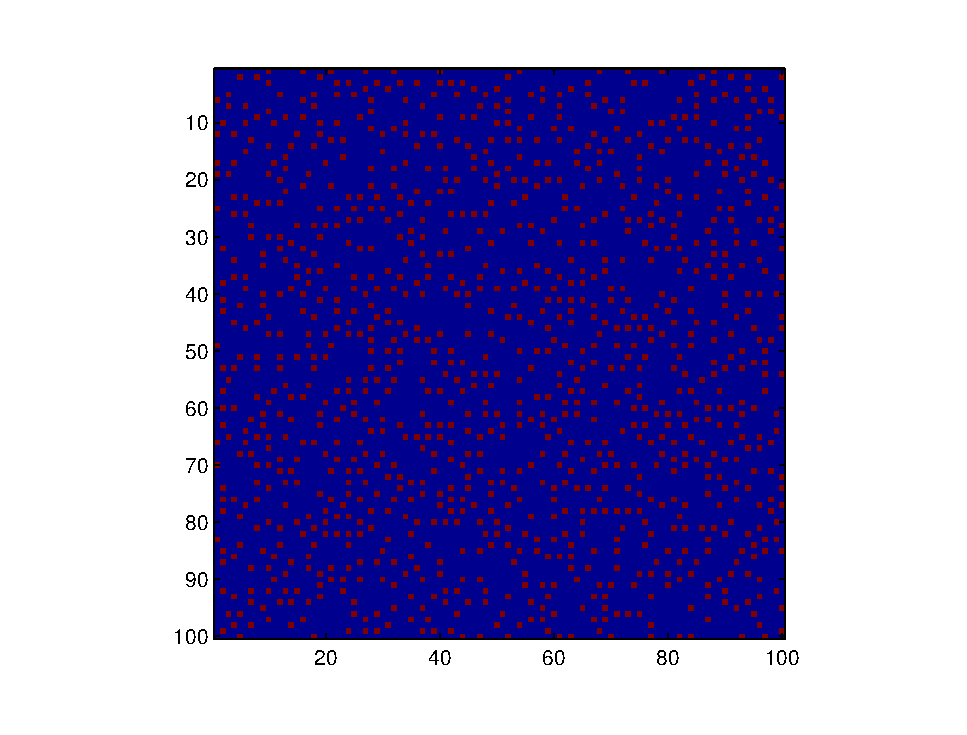
\includegraphics[width=5.5in]{figures/HardCore2D100x100Torus}}
\end{figure}

\begin{simulation}[Glauber dynamics for the hardcore model on a 2D regular torus]
Let us implement a program in \Matlab that will simulate Glauber dynamics to sample uniformly from the harcore configurations on the undirected regular torus graph. 
We can report the sample mean of the fraction of occupied sites on this graph from the simulated sequence and make a movie of the simulaitons (last frame is shown in \hyperref[F:HardCore2D100x100Torus]{Figure~\ref*{F:HardCore2D100x100Torus}}).
\begin{VrbM}
>> HardCore2D
Avg1s =    0.1128
\end{VrbM}
The simulation was implemented in the following M-file:
\VrbMf[label=HardCore2D.m]{scripts/HardCore2D.m}
\end{simulation}


\begin{model}[Ising model]\label{M:GlauberDynamicsIsing}
Let $\Gz = (\Vz,\Ez)$ be an undirected graph.  
The Ising model is a probability distribution on $\Xz = \{-1,+1\}^{\Vz}$, i.e., a way of randomly assigning elements from the set $\{-1,+1\}$ to vertices of $\Gz$.  
The physical interpretation of the model is that each vertex is the position of an atom in a ferromagnetic material and $+1$'s or $-1$'s denote the two possible spin orientations of the atoms.  
There is a parameter $\beta$ in the model called inverse temperature and $\beta \in [0,\infty)$.  
Associated with each spin configuration $x \in \Xz$ is its energy
\[
H(x) = - \sum_{\langle u, v \rangle \in \Ez} x(u) x(v) 
\]
where $x(u)$ and $x(v)$ give the spin orientations of the atoms at vertices $u$ and $v$, respectively.  
So, each edge $\langle u, v \rangle$ adds $1$ to the energy $H(x)$ if its neighbouring vertices have opposite spins and subtracts $1$ from $H(x)$ otherwise.  
Thus, lower energy is equivalent to a higher egreement in spins between neighbouring vertices.  

The Ising model on $\Gz$ at inverse temperature $\beta$ means a random spin configuration $X$ with
\[
\p(X=x) = \pi_{\Gz,\beta}(x) = \frac{1}{\mathcal{Z}_{\Gz,\beta}} \exp{\left(- \beta H(x)\right)} 
=  \frac{1}{\mathcal{Z}_{\Gz,\beta}} \exp{\left(\beta \sum_{\langle u, v \rangle \in \Ez} x(u) x(v)  \right)} \enspace , 
\]
where $\mathcal{Z}_{\Gz,\beta}= \sum_{x \in \Xz}\exp{\left(- \beta H(x)\right)}$ is the normalising constant.
\end{model}

\begin{labwork}[Glauber dynamics for the Ising model on a 2D regular torus]
Implement a program in \Matlab to simulate from the Ising model on the undirected regular torus graph. 
\end{labwork}

Let us explore the physical interpretation of the Ising model further.  
If the inverse temperature $\beta=0$ then we are at infinite temperature and therefore every configuration in $\Xz$ is equally likely, i.e., $\pi_{\Gz,0} = 1/\# \Xz$.  
At the other extreme, if $\beta \to \infty$ then we are approaching zero temperature and the probability over $\Xz$ under $\pi_{\Gz,\infty}$ is equally split between ``all $+1$'' configuration and ``all $-1$'' configuration.  
However, if $\beta > 0$, then we are at some temperature $1/\beta$ that is neither absolutely hot or absolutely cold and therefore the model will favour configurations with lower energy as opposed to higher energy.  Such favourable low energy configurations tend to have neighbouring clumps of identical spins.  
We say that there is a phase transition in $\beta$ since the Ising model's qualitative behaviour depends on whether $\beta$ is above or below a critical threshold $\beta_c$. 

\begin{model}[Proper $q$-colourings]
A proper $q$-colouring of an undirected graph $\Gz=(\Vz,\Ez)$ is an assignment of of $q$ colours labelled $\{1,2,\ldots,q\}$ to vertices in $\Vz$, subject to the constraint that neighbouring vertices do not receive the same colour.  
Let $\Xz$ denote the set of all proper $q$-colourings of $\Gz$.  
If $\Vz$ is large then $\Xz$ can be a large and complicated subset of of $\{1,2,\ldots,q\}^{\Vz}$.  
Note that proper $q$ colourings are a natural generalisation of the hardcore model.
\end{model}


\subsection{Random Walks on $\Zz$ and the reflection principle}
\work

\section{Coupling from the past}



MCMC algorithms make it easy to implement a Markov chain that has a given distribution as its stationary distribution. When used on their own, however, MCMC algorithms can only provide sample values that approximate a desired distribution. To obtain sample values that have a desired distribution {\it exactly} or {\it perfectly}, MCMC algorithms must be used in conjunction with ideas that make clever use of coupling.

MCMC convergence diagnostics based on {\it multiple} independent or {\it coupled} Markov chains running {\it forward} in time have been suggested, but are not completely reliable. The chains are coupled if the same sequence of random numbers is used to propagate all of them. By adopting a different perspective - running multiple coupled chains from the past or {\it backward coupling} - Propp \& Wilson (1996) developed the {\it coupling from the past (CFTP)} algorithm, which allowed exact sample values to be obtained from the stationary distribution of an ergodic Markov chain with {\it finite} state space.

Let us first appreciate the trouble with MCMC algorithms such as Metropolis-Hastings chain, Metropolis chain and Glauber dynamics.  
Firstly, no matter how large we make time $t$ to be we cannot avoid the discrepancy between the $t$-step distribution $\mu_t$ and the stationary distribution$\pi$.  
Consider the following transition probability matrix:
\[
P = 
\bordermatrix{~ & s_1 & s_2 \cr
s_1 & \frac{3}{4} & \frac{1}{4}  \cr
s_2 & \frac{1}{4} & \frac{3}{4} }
\]
We can prove by induction that 
$$\mu_t=\left(\frac{1}{2}\left(1+2^{-t}\right), \frac{1}{2}\left(1-2^{-t}\right)\right)$$
for every $t \in \mathbb{Z}_+$.  
The stationary distribution is $\pi=(1/2,1/2)$.  
So, as $t$ approaches infinity $\mu_t \overset{\mathsf{TV}}{\longrightarrow} \pi$, however for any $t$ the total variation distance between $\dtv(\mu_t,\pi) = 2^{-t}$ is strictly positive.  
Even in this simple example $\mu_t$ may never equal $\pi$ for any finite $t$, however large.
Thus, we have to settle for an approximation to $\pi$ with some acceptable error $\epsilon$.  
Secondly, to make the approximation error measured by $\dtv(\mu_t,\pi)$ smaller than $\epsilon$ we have to find the $\epsilon$-burnin time $\tau_{\epsilon}$ by which $\dtv \left(\mu_{\tau_{\epsilon}},\pi\right) < \epsilon$.  
Determining $\tau_{\epsilon}$ is nontrivial except in special cases and constitutes an active field of research.  




The following material is under \work.
\begin{demo}[Applet -- Perfect sampling.]
The CFTP algorithm starts multiple Markov chains, one for each possible state, at some time $t_0<0$ in the past, and uses coupled transitions to propagate them to time 0. If all the chains {\it coalesce}, (i.e. end up having the same state, at or before time 0), then they will have \textquotedblleft forgotten\textquotedblright their starting values and will evolve as a single chain from that point onwards. The common state at time zero $(X^{(0)})$ is an exact sample value from the stationary distribution. Intuitively, if coalescence occurs at some finite time,$t^{*}<0$, then if the chains had been started in the infinite past, coupling with the same sequence of random numbers will ensure that they coalesce at $t^*$ , and the common chain at time 0 must be stationary because it had been running for an infinitely long time. Thus, the existence of a finite coalescence time can give a stationary sample value in finite time. The use of coupling is essential to induce coalescence in a finite length of time.

Consider a Markov chain with finite state space, $S = {1, 2,\ldots, K}$. The CFTP algorithm starts K Markov chains, one from each state in $S$, at some time $t_0<0$ in the past. A sequence of $t_0$ random vectors, $R^{t+1},R^{t+2},\ldots,R^{0},$, is generated and used to propagate all $K$ Markov chains to time 0. Let $X^{t,k(t_0)}$ represent the state of the Markov chain at time $t$, starting from state $k\in S$ at time $t_0<t$, and let $\phi$ be the update function of the Markov chain, such that:

\begin{equation}
X^{(t+1,k(t_0))}=\phi(X^{(t,k(t_0))},R^{(t+1)})
\end{equation}
\subsection{\alg --{\it Coupling from the past.}}

\begin{tabbing}
Set $t_0=0$.\\
\=Repeat\=\\
		\>\>Set  $t_0=$ $t_0-1$, (take 1 time-step back)\\
		\>\>Generate $R^{(t_0+1)}$ ,\\
		\>\>For $k$\=$=1, 2,\ldots, K$, (for each state)\\
				\>\>\>Set $X^{(t_0,k(t_0))}=k$, (start chain in that state)\\
				\>\>\>For $t$\= $=t_0,t_0+1,\ldots,-1$, (propagate chain to time 0)\\
						\>\>\>\>Set $X^{(t+1,k(t_0))}=\phi(X^{(t,k(t_0))},R^{(t+1)})$.\\
Until $X^{(0,1(t_0))}=X^{(0,2(t_0))}=\Lambda=X^{(0,K(t_0))}$.(check for coalescence at time 0)\\
Return $X^{(0)}$.\\
\end{tabbing}
%\begin{flushright}   $\boxbox$ \end{flushright}
\end{demo}

\begin{example}
Suppose that the Markov chain has the state space, $S = {0, 1, 2}$, and a transition matrix:
$$Q=\left( \begin{array}{ccc}
0.6&0.3&0.1\\
0.4&0.4&0.2\\
0.3&0.4&0.3\\
\end{array}\right)$$

where the $(i, j)$-element is the conditional probability, $P(X^{(t+1)}=j|X^{(t)}=i)$. The matrix of conditional cumulative probabilities is
$$C=\left( \begin{array}{ccc}
0.6&0.9&1\\
0.4&0.8&1\\
0.3&0.7&1\\
\end{array}\right)$$


where the $(i, j)$-element is the probability,  $P(X^{(t+1)}=j|X^{(t)}=i)$. Beginning at $t_0=-1$, three chains are started at 0, 1 and 2. A uniform $(0, 1)$ random number, $U^{(0)}$, is generated (in this example, $R^{(0)}=U^{(0)}$) and used to propagate all three chains to time 0. Suppose that $U^{(0)}\in(0.8,0.9)$. Then the three chains are updated as shown:
\begin{center}
\begin{picture}(60,60)
\put(35,50){$U^{(0)}$}
\put(25,40){2}
\put(55,40){2}
\put(32,45){\vector(1,0){20}}
\put(25,30){1}
\put(55,30){1}
\put(32,35){\vector(2,1){20}}
\put(25,20){0}
\put(55,20){0}
\put(32,25){\vector(2,1){20}}
\put(22,10){-1}
\put(55,10){0}
\put(5,10){$t=$}
\end{picture}
\end{center}
The chains have not coalesced at $t = 0$, so we need to move one time-step back to $t_0=-2$, start three chains at 0, 1 and 2, generate a second uniform $(0, 1)$ random number, $U^{(-1)}$ and use it along with the previous $U^{(0)}$ to propagate the chains to time 0. Suppose that $U^{(-1)}\in(0.3,0.4)$. The three chains then evolve as shown:

\begin{center}
\begin{picture}(100,60)
\put(32,50){$U^{(-1)}$}
\put(25,40){2}
\put(55,40){2}
\put(32,45){\vector(2,-1){20}}
\put(25,30){1}
\put(55,30){1}
\put(32,35){\vector(2,-1){20}}
\put(25,20){0}
\put(55,20){0}
\put(32,25){\vector(1,0){20}}
\put(22,10){-2}
\put(52,10){-1}
\put(65,50){$U^{(0)}$}
\put(85,40){2}
\put(85,30){1}
\put(62,35){\vector(2,1){20}}
\put(85,20){0}
\put(62,25){\vector(2,1){20}}
\put(85,10){0}
\put(5,10){$t=$}
\end{picture}
\end{center}

The chains have still not coalesced at $t = 0$, so we must move another time-step back to $t_0=-3$ and start again, generating a third uniform $(0, 1)$ random number, $U^{(-2)}$. Suppose that  $U^{(-2)}\in(0.3,0.4)$. This is used with  $U^{(-1)}$ and  $U^{(0)}$ from before, giving the following transitions:

\begin{center}
\begin{picture}(130,60)
\put(32,50){$U^{(-2)}$}
\put(25,40){2}
\put(55,40){2}
\put(32,45){\vector(2,-1){20}}
\put(25,30){1}
\put(55,30){1}
\put(32,35){\vector(2,-1){20}}
\put(25,20){0}
\put(55,20){0}
\put(32,25){\vector(1,0){20}}
\put(22,10){-3}
\put(52,10){-2}
\put(62,50){$U^{(-1)}$}
\put(85,40){2}
\put(85,30){1}
\put(62,35){\vector(2,-1){20}}
\put(85,20){0}
\put(62,25){\vector(1,0){20}}
\put(82,10){-1}
\put(95,50){$U^{(0)}$}
\put(115,40){2}
\put(115,30){1}
\put(115,20){0}
\put(92,25){\vector(2,1){20}}
\put(115,10){0}
\put(5,10){$t=$}
\end{picture}
\end{center}
All three chains have now coalesced at $t = 0$ and so $X^{(0)}=1$ is accepted as a sample value from the stationary distribution. The whole process is repeated to get another independent sample value. It is important to note that even though the chains have coalesced at $t =  1$, with the common value $X^{(-1)}=0$; this value at the time of coalescence is not accepted as being from the stationary distribution. This is because the time of coalescence is a random time that depends only on the sequence of random numbers, $U^{(0)},U^{(-1)},\ldots$; while the time at which a coalesced state has the required stationary distribution must be a fixed time. In the CFTP algorithm, this {\it fixed} time has been arbitrarily specified to be $t = 0$.
\end{example}

\begin{example}
To see that the state at the time of coalescence does not have the stationary distribution, suppose that the state space is $S = {1, 2}$ and the transition matrix is:
$$Q=\left(
\begin{array}{cc}
0.5 &0.5 \\
1 &0 \\ 
\end{array}\right).$$


Since $Q(2, 1) = 1$, the two coupled chains must be in state 1 at the time of coalescence. However, the stationary distribution of this Markov chain is $f(1) = 2/3$ and $f(2) = 1/3$, and so the state at the time of coalescence cannot be from the stationary distribution.
\end{example}

Instead of taking a single step back when the two bounding chains fail to coalesce, any decreasing sequence of time-steps may be used. The \textquotedblleft double-until-overshoot" choice of $t_0=-2^0,-2^1,-2^2,\ldots$ is optimal in the sense that it minimises the worst-case number of steps and almost minimises the expected number of steps for coalescence.


\begin{exercise}
Implement the CFTP algorithm for the Markov chain in Example 2.5.3 and use it to generate 1000 sample points from the stationary distribution of the chain. The stationary distribution can be shown to be:
$$\begin{array}{|c|c|c|c|}\hline
x	&0&	1&	2\\ \hline
f(x)	&0.4789	&0.3521	&0.1690\\ \hline
\end{array}$$
Compare the relative frequencies of the generated sample with the true stationary probabilities.

\end{exercise}

\begin{exercise}
2.6.19	Consider a Markov chain with a state space $S = {0, 1, 2, 3}$ and the transition matrix:
$$Q=\left( \begin{array}{cccc}
0.6&0.4&0&0\\
0.4&0.2&0.4&0\\
0.2&0.4&0&0.4\\
0&0.2&0.4&0.4\\
\end{array}\right).$$

Let $f=(f_0,f_1,f_2,f_3)$ be a row vector containing the stationary probabilities of the chain.
\begin{asparaenum}[(a)]
\item By solving $fQ=f$ and $f_0+f_1+f_2+f_3=1$ simultaneously, show that the stationary distribution of the chain is $f=(14/35,11/35,6/35,4/35)$.

\item Implement the \textquotedblleft double-until-overshoot" version of the CFTP algorithm to generate from the stationary distribution, and use it to obtain 1000 sample points. Compare the relative frequencies of the generated sample with the true stationary probabilities.
\end{asparaenum}
\end{exercise}
